\documentclass[a4paper]{article}
%\usepackage{fourier-otf}
\usepackage[utf8]{inputenc}
\usepackage{graphicx}
\usepackage{algorithm}
\usepackage{algpseudocode}
\usepackage{float}
\usepackage{lipsum}
\usepackage{scrextend}
\usepackage{biblatex}
\addbibresource{bibliography.bib}
\usepackage{listings}
\usepackage{amsmath}
\usepackage{amsfonts}
%\usepackage[square,sort,comma,numbers]{natbib}
\newtheorem{theorem}{Theorem}[section]
\usepackage{color}
\usepackage{makeidx}
\usepackage{titlepic}
\definecolor{mygreen}{rgb}{0,0.6,0}
\definecolor{mygray}{rgb}{0.5,0.5,0.5}
\definecolor{mymauve}{rgb}{0.58,0,0.82}
\lstset{ %
	backgroundcolor=\color{white},   % choose the background color
	basicstyle=\footnotesize,        % size of fonts used for the code
	breaklines=true,                 % automatic line breaking only at whitespace
	captionpos=b,                    % sets the caption-position to bottom
	commentstyle=\color{mygreen},    % comment style
	escapeinside={\%*}{*)},          % if you want to add LaTeX within your code
	keywordstyle=\color{blue},       % keyword style
	stringstyle=\color{mymauve},     % string literal style
}
\usepackage{hyperref}
\hypersetup{
  colorlinks   = true,    % Colours links instead of ugly boxes
  urlcolor     = black,    % Colour for external hyperlinks
  linkcolor    = black,    % Colour of internal links
  citecolor    = black      % Colour of citations
}
%\title{First chapter}

%\author{F.Bernardi}

%\protect\\ 

\newcommand{\myName}{Fabrizio Bernardi}
\newcommand{\myTitle}{Data analysis and modeling of calcium activity in   mice somatostatin neurons}
\newcommand{\myDegree}{Programme: \protect\\ \textit{Mathematical Engineering}}
\newcommand{\myCycle}{XXXI cycle}
\newcommand{\myDepartment}{Department of Mathematics}
\newcommand{\myUni}{Politecnico di Milano}
\newcommand{\myYear}{2022}
\newcommand{\myTime}{01 Jan \myYear}

\pdfbookmark{Cover}{cover}





\begin{document}
	%	\maketitle
		
	

	
	
	
	
	\clearpage
	
	\begin{titlepage}
			\begin{minipage}{\linewidth}
			\centering
			\begin{minipage}{0.45\linewidth}
				\begin{figure}[H]
					
\includegraphics[width=\linewidth]{Logo_IIT.png}
					
				\end{figure}
			\end{minipage}
			\hspace{0.05\linewidth}
			\begin{minipage}{0.45\linewidth}
				\begin{figure}[H]
					
\includegraphics[width=\linewidth]{Logo_Politecnico_Milano.jpg}
					
				\end{figure}
			\end{minipage}
		\end{minipage}
		
		\begin{addmargin}[1cm]{-1cm}
			\setlength{\parindent}{0pt}
			\vfill
			
			{\huge\bfseries\myTitle}
			
			\vspace{2cm}
			
			{\Large M.Sc. Thesis of\\[0.125cm]}
			{\LARGE\bfseries\myName}
			
			\vspace{1cm}
			
			\large
			Supervisor:\\[0.125cm]
			{\Large Prof. Riccardo Sacco}
			
			\vspace{0.5cm}
			
			\large
			Co-supervisors:\\[0.125cm]
			{\Large Dr. Francesco Papaleo \\
			Dr. Greta Chiaravalli}
			
			\vspace{2cm}
			
			\myDegree
			
			\vspace{0.5cm}
			
			\myDepartment \\
			\myUni
			
			\vfill
		\end{addmargin}
	\end{titlepage}
	
	\tableofcontents
	
	\newpage
	
	\section{Neurobiology of behaviour}
	
	
	In this first chapter, the biological and experimental foundations of this work will be presented. After a brief review of the main notions of neurobiology, such as the structure of a neuron, the propagation of an action potential in neuronal circuits and the intracellular calcium dynamics, there will be a closer focus on the areas of the brain that are involved in the following discussions.\\
	Next, the experimental setup for such studies is presented, through the description of the behavioral tasks performed on mice and the experimental techniques for calcium imaging, from which it will be possible to extract the data analyzed in Chapter 2.\\
	Finally, a  quite modern and extremely relevant topic for this work is introduced: the synchronization among neural signals.
	
	\subsection{Neuronal circuits to describe behaviour}
	
	\begin{figure}[H]
		\begin{center}
			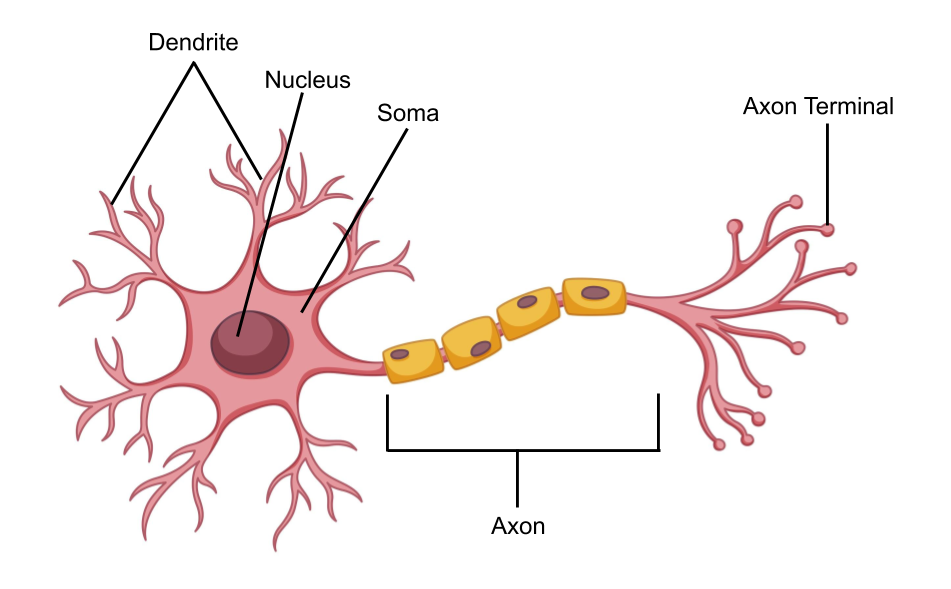
\includegraphics[scale=.25]{neuron.png} 
		\end{center} 
		\caption{\textit{Schematic representation of a neuron}}
		
	\end{figure}
	
	The importance of the brain in mammals is by today extremely evident: this vital organ allows us to think,  to capture the stimuli from the environment and elaborate them, enriching our memory and  our learning. The brain is the control center of our movements and our actions, it allows us to speak, to understand other individuals and elaborate responses. Most importantly for this work, however, the brain, from its basic cellular units, can explain our behaviour and our emotions. \\

	
	The brain itself is part of the \textbf{nervous system (NS)}, and its most important cell is the \textbf{neuron}.	Neurons are one of the basic unit needed for the transmission of
	the electric signals, both within the same area and between different areas of
	the brain, allowing the NS to collect information and to react to stimuli,
	elaborating decisions based on them. \\
	The neuron is composed of a central body called \textit{soma}, of the \textit{dendrites}, cellular extensions which collect stimuli from near areas, and of the \textit{axon}, the biological cable connecting one neuron to another, in order to propagate information. 
	Another type of cells present in the NS are the \textbf{glial cells} (like astrocytes), which perform functions of protection, sustainment and nutrition for the neurons. Although glial cells are not the main focus of this work, their contribution should not be neglected, as it has been shown to be relevant in many important processes of the nervous system [Semyanov, Henneberger 2020]. \\
	
		
	
	Neurons are \textbf{excitable} and \textbf{conductive}, i.e. they can generate an electrical impulse and transmit it to other neurons, forming neuronal microcircuits, often associated with a specific area and/or task of the brain. \\
	Inside every neuron, in the cytoplasm, there is a coexistence of different ionic species (mostly $Na^+, Cl^-, K^+, Ca^{2+}$) which, in equilibrium conditions, assume a certain concentration, which conurs to determine a difference between the electric potential assumed inside and outside the cell: we call this quantity the \textbf{membrane potential} of the cell (indeed it is the potential drop formed across the cell's membrane).  In reaction to an external stimulus, the ionic concentrations change rapidly their values, provoking a heavy change in the membrane potential. As a consequence, the excitation of a neuron happens, as well as the formation of an \textbf{action potential}, which will propagate to other neurons across the axon. 
\begin{figure}[H]
	\begin{minipage}{\linewidth}
		\centering
		\begin{minipage}{0.45\linewidth}
			\begin{figure}[H]
				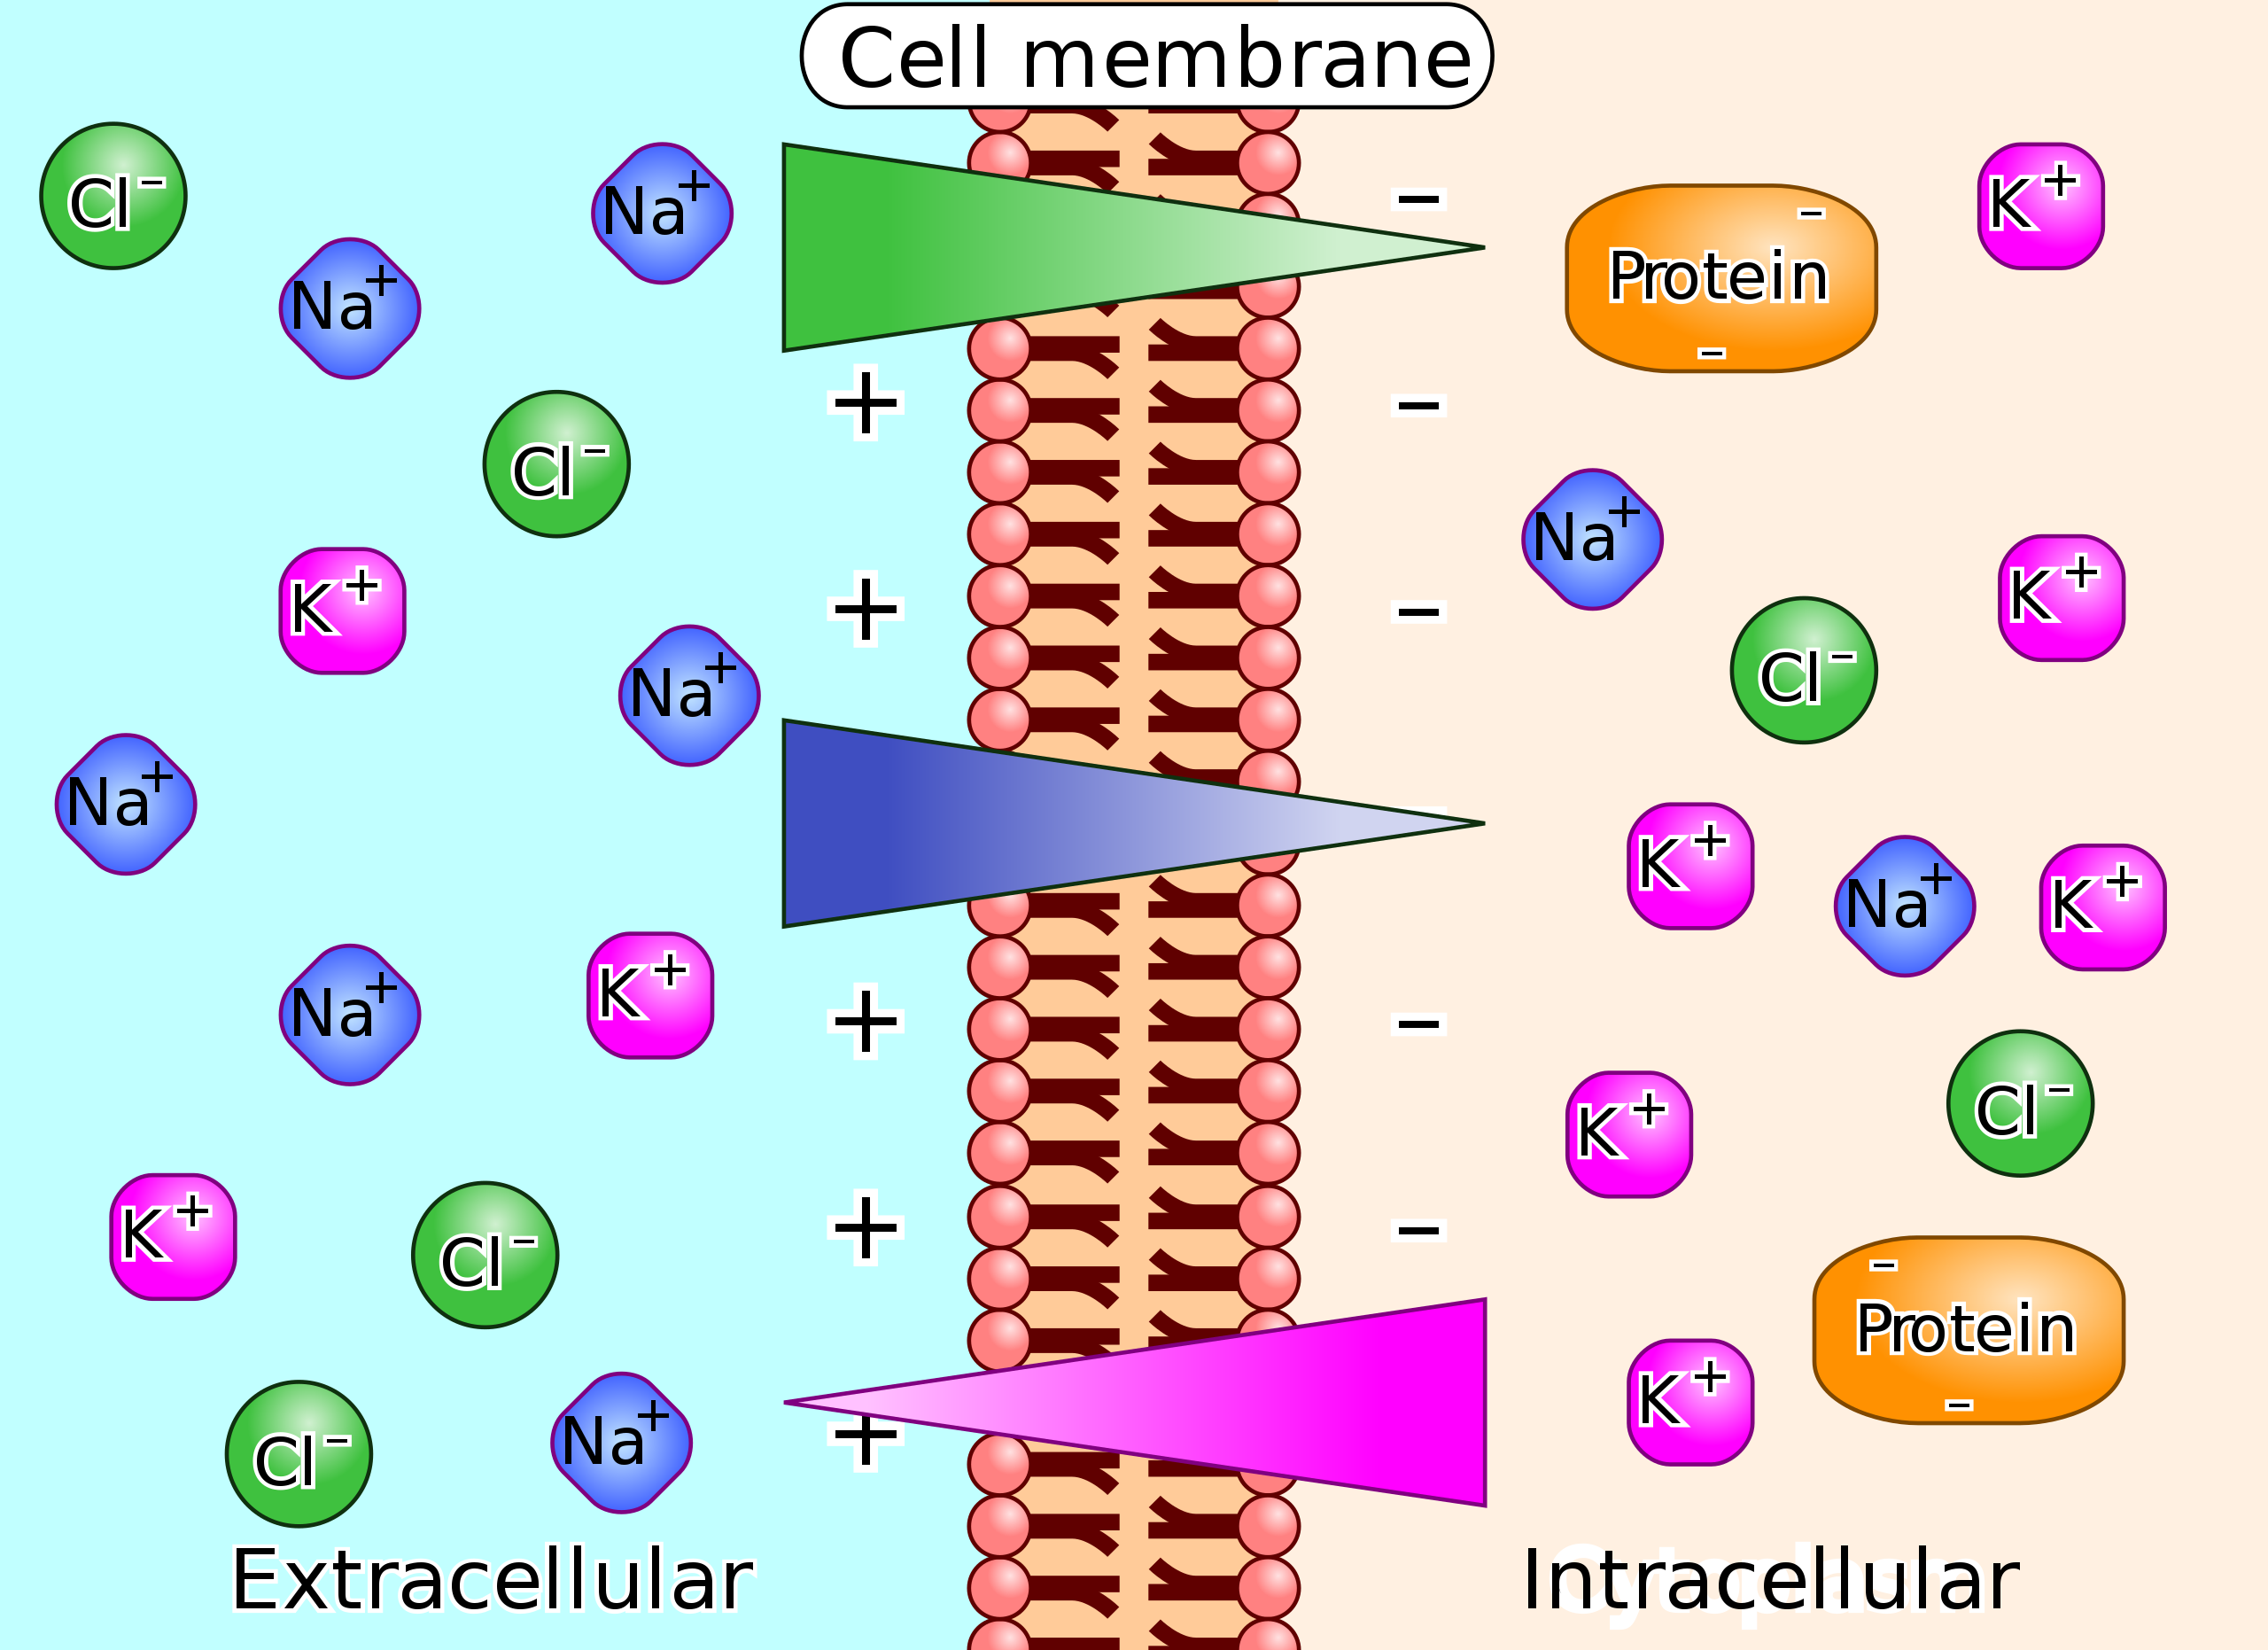
\includegraphics[width=\linewidth]{AP1.png}
				
			\end{figure}
		\end{minipage}
		\hspace{0.05\linewidth}
		\begin{minipage}{0.45\linewidth}
			\begin{figure}[H]
				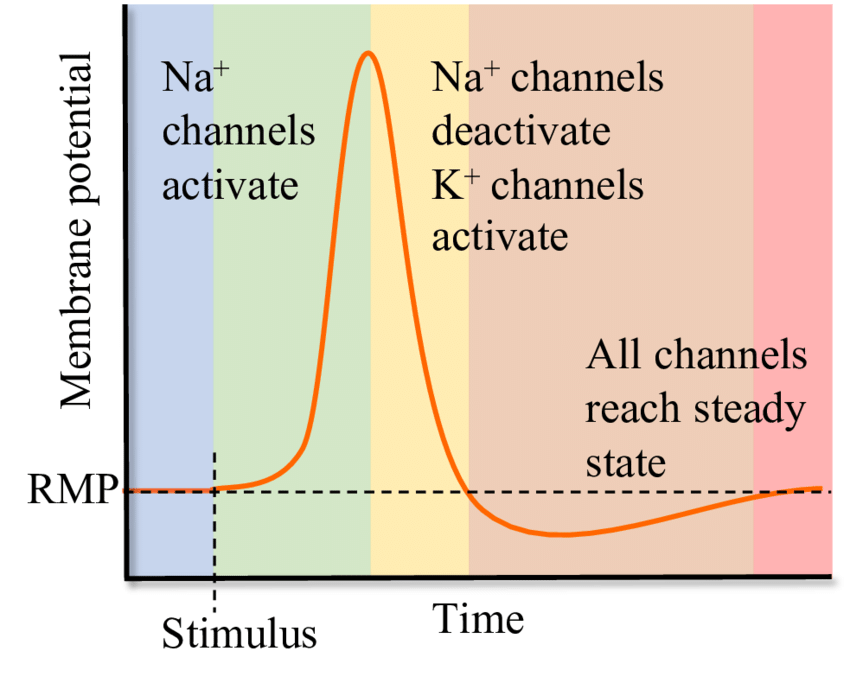
\includegraphics[width=\linewidth]{AP2.png}
				
			\end{figure}
		\end{minipage}
		
	\end{minipage}
\caption{\textit{Left: schematic representation of ionic species inside and outside the cellular membrane. Such species are allowed to pass through the membrane only in specific circumstances through adhibited ionic gates \\
Right: example of action potential formation in reaction to a stimulus}}
\end{figure}

At the end of the axon, the link between a neuron and its neighbour, and the relative passage of the electrical impulse, happens thanks to a chemical \textbf{synapse}, a particular structure located in the terminal of the axon. Here, special molecules called \textit{neurotransmitters} are syntethized, and the arrival of an action potential allows such molecules to travel towards the \textit{intersynaptic space}, where they can bind to receptors located in the post-synaptic cell. The response of the post-synaptic cell, then, can be either excitatory or inhibitory, based on whether the impulse is preserved in the circuit or supressed.\\
The synapses (and thus their corresponding neuron) can be classified in four main groups, depending on the type of neurotransmitter which they release:  glutamatergic, GABAergic, cholinergic,  adrenergic. The most relevant for this work will be the one of GABAergic synapses, consisting of inhibitory neurotransmitters which reduce the excitability of the neurons.
\begin{figure}[H]
	\begin{center}
		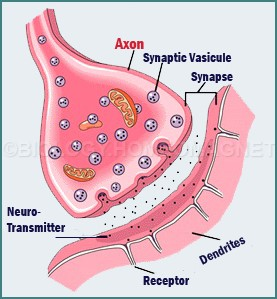
\includegraphics[scale=1.6]{synapse.jpg} 
	\end{center} 
	\caption{\textit{Schematic representation of a chemical synapse}}
	
\end{figure}



In neurobiology, the conditions under which a neuron can be considered \textbf{active} are not unique and matter of debate; in the context of neural activity, the literature usually means either the already discussed electrical activity, or the \textbf{calcium activity}. The intracellular dynamic of this particular element, in ionic form of $Ca^{2+}$, is known to be essential for the main cellular processes, and is strictly related to the formation of an action potential and subsequent propagation of the electrical impulse.\\
 Indeed, we can usually observe  \textit{strong instabilities} in the intracellular calcium concentration, which often show fast oscillations and changes, through the formation of sudden peaks: we will define the neuron as \textit{active} in correspondence to these peaks.

\begin{figure}[H]
	\begin{center}
		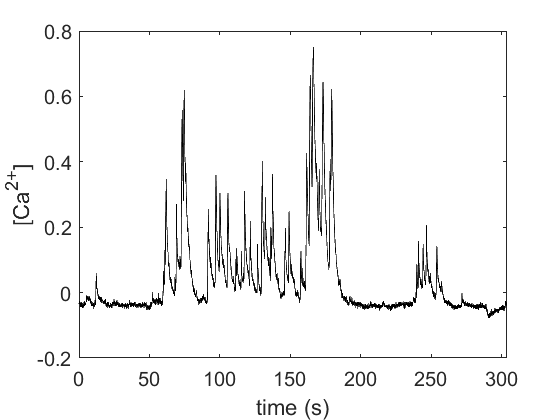
\includegraphics[scale=.50]{Ca_conc.png} 
	\end{center} 
	\caption{\textit{Example of $Ca^{2+}$ concentration recorded in a neuron, as function of time}}
		
	\end{figure}
	
	Having defined the meaning of neuronal activity, we can ask ourselves whether this activity could be related to aspects like behaviour, emotion, body language, mood: in other words, to investigate whether there is a connection between the activation of some specific neurons, and what animals do.\\
	This topic has fascinated neuroscientists for decades, and from what it has been discovered so far, it seems evident that \textbf{different brain circuits are responsible for different behaviours} (although these distinctions may not always be that marked, unique and easy to detect).

	
	The neurobiology experiments on which this work relies on refer mainly to some particular areas of the brain, which previous studies found to be strictly connected to emotional and behavioral processes [Etkin et al. 2011]:
	\begin{itemize}
		
		\item \textbf{Medial prefrontal cortex (mPFC)}:  part of the frontal cortex, the area of the brain located in the frontal lobe. This area is implicated in cognition processes, including socio cognitive abilities,  with strong connections with decision making [Carlen 2017]
		
		\item \textbf{Anterior Cingulate Cortex (ACC)}: part of the cingulate cortex and situated in proximity of the mPFC,  with which  ACC shares a lot of functionalities. Indeed, experimental evidence of the connection between this area of the brain and emotions have been found [Zheng 2020]. This area seems also to be implicated in social aspects like morality or empathy [Carillo 2019], as reaction to interactions with another individual
		
		\item \textbf{Amygdala}: nuclear complex located in the medial part of the temporal lobe. It is responsible for the elaboration of the emotions, it collects stimuli from the thalamus and elaborate responses: in other words, it plays the role of emotional thermometer of the body and the decision maker for adequate responses [ARTICOLO?]
	\end{itemize}


	
	\begin{figure}[H]
		\begin{center}
			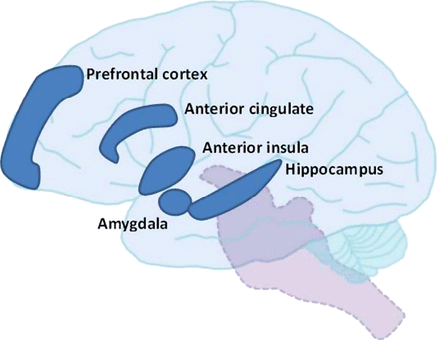
\includegraphics[scale=.55]{brain.png} 
		\end{center} 
		\caption{\textit{Main areas of the brain involved in behaviour and emotion recognition}}
		
	\end{figure}

\newpage

\subsection{In vivo studies on mice}

According to the \textit{Foundation of Biomedical Research (FMR)}, approximately $95\% $ of all lab animals are mice or rats, as in the case of this current work. Although very often the final goal of the research is an application useful for humans, the reasons why mice are the first choice for experiments are numerous. First of all, mice are mammals quite similar to humans when it concerns genetics, at the point that scientists have been able to reproduce genes in mice similar to the ones implied in human diseases ("\textit{transgenic mice}" [Harari,Abramovich 2014]); rodents, indeed, are also easy to manipulate from a genetic point of view. Another reason is definitely the fact that mice are small, easy to control, quite cheap to buy and usually docile. Finally, being the most used animal in research, the largest information and literature which can be found is about them, their anatomy, their typical behaviours, and by today large populations of rodents have been created and used exclusively for experimental purposes, being almost all identical and therefore setting a uniform standard for study and validation of results. \\
Through a  \textbf{behavioral task}, one or more mice are put in a particular situation designed to study their reactions, such as a shown behaviour or movement, and, in this context, the goal is to find a relationship with their correspondent neural activity. Therefore, the overall experiment consists in the following steps:
\begin{enumerate}
	\item Preparation of the arena and equipment for the task 
	\item Preparation of the mice for the experiment, both in terms of behavioral conditioning, and for neural activity measurments
	\item Performance of the test with simultaneous recordings of  aspects of interest such as behaviour or neuronal activity
	\item Pre-processing and analysis of the collected data
\end{enumerate}

\begin{figure}
	\begin{center}
		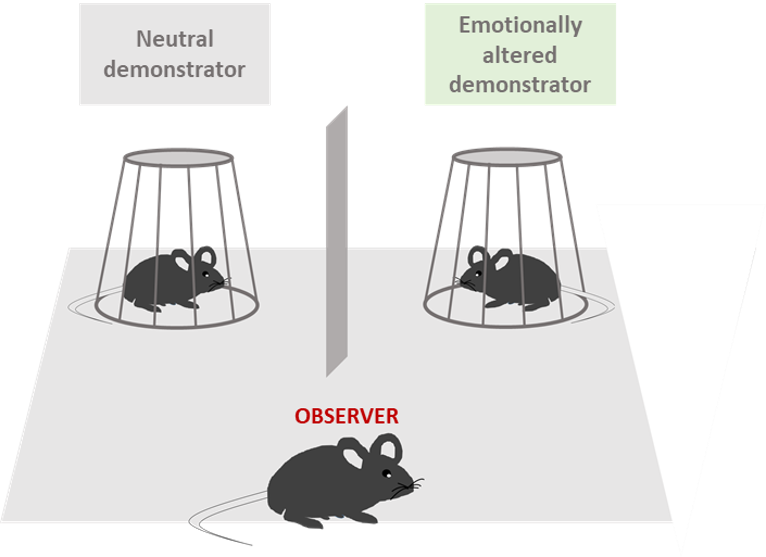
\includegraphics[scale=.60]{mice_task.png} 
	\end{center} 
	\caption{\textit{Basic setting of the emotion discrimination task: one mouse (the \textit{observer}) is free to move in the arena, while the others two (the \textit{demonstrators}) remain inside a cage. One of the demonstrators has a neutral affective state, the other an altered affective state}}
	
\end{figure}
In this work, the behavioural task which has been studied is a particular realization of the \textbf{emotion discrimination task}. The first step of these types of tasks, performed in this way several times in the past, sees the presence of three mice: one, called the \textbf{observer}, is a mouse free to move in an arena, while the others two, called the \textbf{demonstrators}, remain in a cage. In the phase preceding the test, the \textit{habituation phase}, one of the two demonstrators is \textit{emotionally altered}: namely, it is subjected to specific conditions and procedures which provoke an alteration of its affective state. This alteration could be either negative (usually stress condition following a 15-minutes period of restrain) or positive (usually relief condition, consisting in water \textit{ad libitum} following water deprivation). The other demonstrator and the observer are instead in a \textit{neutral} state.\\

Previous works on this setup [Scheggia-Managò] were performed using both positively and negatively affected demonstrators. The cellular target consisted in a specific subpopulation of neurons, which is thought to be involved in processes like \textit{affective state discrimination}: the \textbf{somatostatin (SOM+)} interneurons in the medial prefrontal cortex.\\
These neurons, expressing the somatostatin neurotransmitter, form a small
subgroup, distinct from others like pyramidal neurons or parvalbumin interneurons, but unlike these former ones, they seem to be directly implicated in the affective state discrimination of a conspecific mouse. The data analysis on the task showed some remarkable results:

 \begin{itemize}
 	
 	\item The time spent by the observer near the altered demonstrator was significantly higher than the time spent near the neutral demonstrator. A similar consideration holds for the duration of the moments when reciprocal sniffing between two close mice happened
 	
 	\item This  discrimination appears to be stronger in the first period of the test
 	
 	\item The discrimination is directly connected to the presence of a mouse in an altered state (both negative and positive), since from the repetition of the task using only two neutral demonstrators no significant differences emerged
 	
 	\item By repeating the task elinitaing one sense at a time, it has been shown that the main sense responsible for the discrimination is olfaction. However, in order to achieve the same results of the test, a combination of both olfactory and visual cues is needed
 	
 	
 	\item The neural activity of the observer (both in terms of electrical impulse and  calcium peaks) showed stronger values during the interactions with the altered mouse rather than the neutral one
 	
 	\item If optoenetic inhibition of SOM+ cells [REFERENCE?] is
 	performed on the observer before the test, the discrimination disappears, namely no relevant differences between time spent and sniffing behaviour have been observed in relation to the altered demonstrator rather than the neutral one
 	
 	
 	\item All the previous considerations do not apply to other neuronal categories like pyramidal or parvalbumin interneurons
 	 
 \end{itemize}
 
 Overall, these results seem to show a \textbf{key role of the somatostatin interneurons in affective state discrimination}.

	\begin{figure}
	\begin{center}
		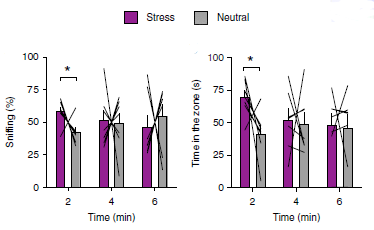
\includegraphics[scale=.99]{scheggia.png} 
	\end{center} 
	\caption{\textit{Recording of sniffing times (left) and proximity times (right) between observer mouse and stressed demonstrator}}
	
\end{figure}


Other examples of emotion discrimination in mice related to SOM+ interneurons can be found in [Mariotti et al 2018], with a focus on their effect on cortical astrocytes: the main result shown in the study consist in a \textbf{crucial role of somatostatin} in the stimulation of responses by astrocytes.\\
As a first result, it has been shown that the stimulation of SOM+ interneurons (via 10-pulses light stimulation of calcium indicators), increases the $Ca^{2+}$ response from astrocytes. Also in this case, a comparison with parvalbumin (PV+) interneurons show the \textit{critical sensitivity of astrocytes only to SOM+ interneurons, but not PV+}. Overall, this study reveals that a sustained activity in the SOM+ interneuron circuits is complemented by
a sustained activity in the astrocytic network, thus confirming the importance of astrocytes and their link to inhibitory neuronal circuits. 
\\

Somatostatin interneurons are not the only neuropeptide that has been shown to be linked to emotion discrimination. For example, in [Ferretti-Maltese 2018], the in vivo task on mice targets the \textbf{oxytocin (OXT)} neurotransmitter, studying its release in the central amygdala. The behavioral task of this study has a similar structure to [Scheggia-Manago], in which neutral and altered demonstrators were contraposed to an observer mouse. Also this case shows evidence of  discrimination caused by the altered mouse (for example,through an increased sniffing activity), as well as the importance of olfactory clues in the process of such discrimination.\\
A reduction of  OXT level in the central amygdala resulted in the \textit{abolishment} of emotion discrimination, while a new increase of such level resulted in the rescue of the former conditions, thus remarking the central role of the OXT neuropeptide in the emotion discrimination.
\\

When targeting a specific neuronal subpopulation, the hope is to always find  more evidence on its connection with  properly shown tendencies, emotions or behaviors that are common to known diseases. In the case of the emotion discrimination task targeting SOM+ interneurons in the mPFC, for example, the observed effects in the abolition of discrimination, following photoinhibition of such neurons, could be similar to the ones observed in neurodevelopmental disorders such as autism spectrum disorders (ASDs) or schizophrenia. Therefore, this approach aims to investigate the causes of a specific issue at a basic and detailed level such the one of single neuron precision, with the ultimate goal of acting on such level to perform a change on the macroscopic effects.\\
In order to do so, the paradigm of the task has to be defined in a way that it allows a collection of unbiased results, but an adequate way to perform an imaging of the neuronal activity of interest is necessary as well (and described in the following sections). As a final step, a proper data analysis on those results has to be performed (Chapter 2).


\subsection{Calcium imaging through Inscopix}



\begin{figure}[H]
	\begin{center}
		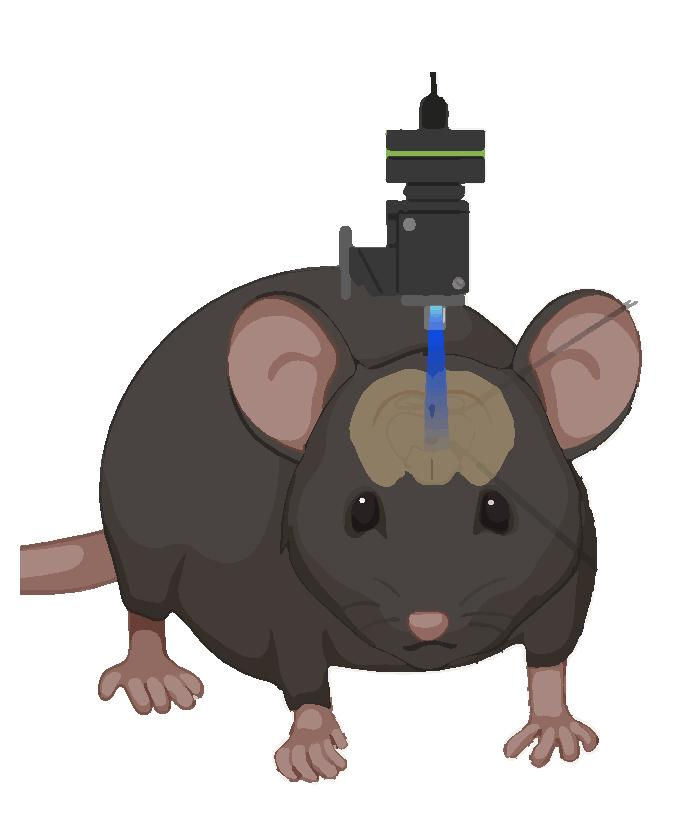
\includegraphics[scale=.35]{Inscopix.jpg} 
	\end{center} 
	\caption{\textit{The Inscopix miniscope}}
	
\end{figure}


In this section, a powerful tool for single neuron calcium imaging will be presented. The Inscopix company [https://www.inscopix.com/] provides tools and software to extract calcium tracks as one photon measurements from in vivo experiments on mice.\\
To measure the intracellular $Ca^{2+}$ concentration in a single mouse during a behavioral task, the first step is the performance of a surgery on the mouse to implant a miniscope in the \textit{region of interest (ROI)} of the brain to be investigated. On the same mouse, \textbf{genetically encoded calcium indicators (GECI)}, such as the \textbf{GCaMP} protein, are adopted. These types of proteins, when bound to $Ca^{2+}$, emit a fluorescent light, which intensity will be captured by the miniscope. At the end of the test, the miniscope will be able to give back a video of the ROI, in which the evolution of the fluorescence through time can be appreciated  in the neurons. In this way, it is possible to obtain a representation of the intracellular calcium oscillations behaviour during the whole task. This information can be combined with behavioral or positional data of the mice in the arena, making it possible to start a data analysis and look for correlations between behaviour and neural activity.\\
In order to have the data ready to be analyzed, however, the Inscopix software manages also the pre-processing part, which goes through the following steps:

\begin{figure}[H]
	\begin{center}
		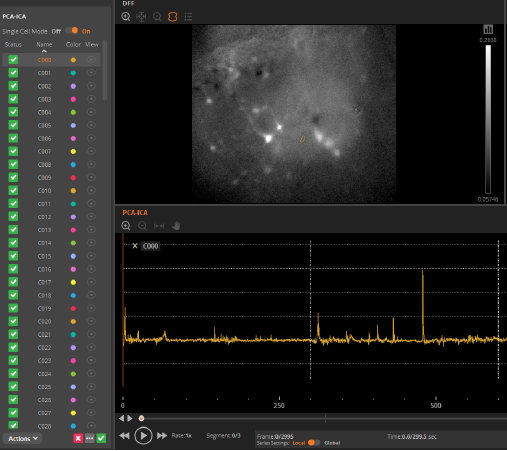
\includegraphics[scale=.70]{Inscopix2.png} 
	\end{center} 
	\caption{\textit{Example of pre-processing work through Inscopix software. We can appreciate: the list of detected neurons (left), a segment of the video in the ROI (top-right) and an example of the calcium track recorded in a single neuron through time (bottom-right)}}
	
\end{figure}

\begin{enumerate}
	
	\item If needed, more videos recorded from the test can be combined, in order to obtain a single final video of the ROI through time
	
	\item \textbf{Spatial and temporal downsampling} are performed, selecting the appropriate scale factors of space and time which allow to capture all the important information
	
	\item \textbf{Spatial filtering} of the image: it removes low and high frequencies with a bandpass filtering. The filter has the form
	
	$$ M_f^{band} = GB(M_f,\sigma_{high}) - GB(M_f,\sigma_{low})$$
	
	Where $M_f$  represents the frame $f$ of movie $M$, $GB$ is the \textit{Gaussian Blur} function, and the standard deviations $ \sigma_i = \frac{2 ln(2)}{2 \pi \lambda_i}$ are computed from the cut-off values $ \lambda_{high}$ and $ \lambda_{low}$
	
	\item \textbf{Motion correction}: it accounts for the motions between different frames of the videos, applying a correction to let every pixel staying at the same place along the different frames of the movie
	
	\item \textbf{Pixel normalization}: each pixel of a frame represents a different luminosity, caused by the fluorescence obtained from the reaction with the GCaMP. After the preprocessing, the value of the fluorescence (which estimates the calcium concentration) is expressed as 
	$$\frac{\Delta F }{F} = \frac{F(x,y,t) - F_b}{F_b}$$
	where $F(x,y,t)$ represents the measured fluorescence at the point $(x,y)$ at time $t$, while $F_b$ is a baseline fluorescence value (usually the mean value of the movie, in some cases the minimum). After this step, the returned value for every pixel is an adimensional relative value of fluorescence
	
	\item The \textbf{PCA-ICA algorithm} attempts to recognize the neurons of the ROI in the movie. Based on given information such as average cell's diameter, a principal component analysis (PCA) is performed, followed by an independent component analysis (ICA), until convergence. In particular, the frames of the movie, represented as matrices, are rasterized into 1D vectors and they are normalized on mean and standard deviation. At this point, a principal component analysis is performed, in order to reduce dimensionality. Every frame is then approximated by a weighted sum of the principal trace components. Finally, an ICA algorithm is launched. At the end of this process, every neuron will be identified, labeled, and gifted with a calcium activity value (which is actually  $\frac{\Delta F }{F}$) for every time instant of the movie. 
	
	\item \textbf{Final adjustements}: appropriate algorithms or manual fixing are performed to take into account some imperfections, such as mistakes in neuron identification, inaccuracies due to overlapping neurons, excessive noise in the calcium traces for a neuron (discarding the corresponding cell from the analysis)
	
	\item \textbf{Data import}: finally, data are imported in a csv file and are ready to be analyzed (in this work, using the software \textsc{Matlab})
	
\end{enumerate} 


At the end of all these steps, the final data available consist of a list of every neuron detected, in which for every one of them, at every time stamp is associated the corresponding value of $\frac{\Delta F }{F}$ recorded. The preprocessing step is now over, and the calcium traces of every neuron in the ROI are available for the data analysis process.	


\newpage
\subsection{Calcium imaging through Fiberphotometry}

\begin{figure}[H]
	\begin{center}
		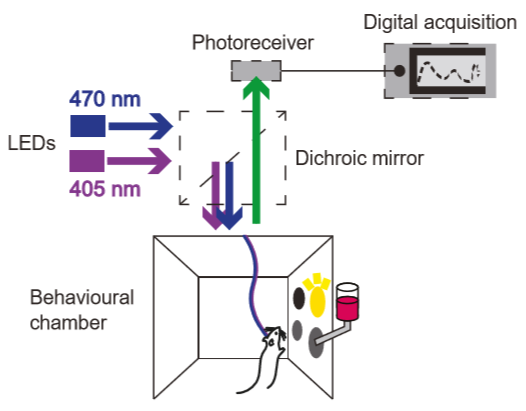
\includegraphics[scale=.50]{fiberphotometry.png} 
	\end{center} 
	\caption{\textit{Fiberphotometry experimental setup}}
	
\end{figure}

In the previous section, it has been shown a calcium imaging technique based on single neuron traces measured with single photon miniscopes. In this section, another common technique for calcium imaging will be presented: \textbf{fiberphotometry}. \\
The main goal of this technique is the same as the Inscopix imaging one, however technical equipment, methodology and results present substantial differences.\\
Relying on genetically encoded calcium indicators such as GCaMP, with fiberphotometry the fluorescence signal is recorded through \textit{optic fibers}, typically of length $300-400 \mu m$. An excitation of GCaMP is performed using a blu LED light at the appropriate wavelength ($470 nm$), which is transmitted through the optical cannula implanted in the mouse, while an emission green light ($525 nm$) is relayed to a photoreceiver. Often, a second excitation light (violet, $405 nm$), is used as well, to take into account autofluorescence and produce an isosbestic (calcium-independent) control signal [TESI PHD GIULIA].\\
 Finally, a software manages the output signal in order to perform filtering and return a collective raw signal, separating the two contributions from blu and violet lights. Such signal, unlike the miniscope neuronal imaging, can only be an \textit{aggregate} signal of the observed area. This implies that the fiberphotometry technique produces signals at lower spatial resolution than the previously introduced technique. However, this technique is becomingincreasingly popular because its smaller accuracy is compensated by several positive factors:

\begin{itemize}
	
	\item The overall experimental setup for fiberphotometry results cheaper than the one for miniscope imaging 
	
	\item The procedure operated in mice are less invasive, and the subjects are more suitable to long freely behaving experiments
	
	\item The implant of the cannula is relatively easy to perform, and a good signal is collected even with fiber placements in the neighborhood of GECI -expressing populations [Siciliano and Tie 2018]
	
	\item Multiple areas of the brain can be investigated at the same time 
	
	\item Fiberphotometry can be used for other fluorescent indicators, such as norepinephrine (Feng et al., 2019), GABA (Marvin et al., 2019), glutamate (Liang et al., 2015),
	acetylcholine (Jing et al., 2018) and dopamine (Patriarchi et al., 2018)
	
	
	
\end{itemize}


\subsection{Synchronization of neural activities}

\begin{figure}[H]
	\begin{minipage}{\linewidth}
		\centering
		\begin{minipage}{0.6\linewidth}
			\begin{figure}[H]
				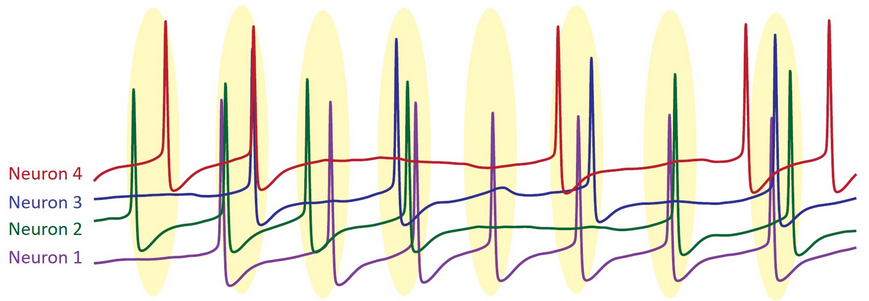
\includegraphics[width=\linewidth]{synch.png}
				
			\end{figure}
		\end{minipage}
		\hspace{0.05\linewidth}
		\begin{minipage}{0.6\linewidth}
			\begin{figure}[H]
				\includegraphics[width=\linewidth]{Intebrain.png}
				
			\end{figure}
		\end{minipage}
		
	\end{minipage}
\caption{\textit{Top: single neuron synchronization \\
		Bottom: overall activity synchronization}}
\end{figure}

In the previous sections, the concept of \textit{neural activity} has been introduced in its different shapes. Not only it can be identified with the electrical and calcium activity, but activity necessarily refers to a specific area: it can be the activity of a single neuron or of a group of neurons in a ROI (often, in this case, the activity is attributed to the whole animal for that specific context). in any case, the main object of interest of neural activity is a \textbf{signal evolving in time}.\\
While historically the study of neural activity has been mostly dealing with individuAL signals treated one by one, the focus, in the most recent years, is extending to cover as well a more complex topic: the \textbf{synchronization between different brain activities}. The definition of synchronization between signals, not unique and assuming different shapes for different needs (Chapter 2), can involve two types of correlations:

\begin{itemize}
	
	\item \textbf{Intraneuronal synchronization}: the signals of  single neurons show a correlated activity. Often (but not necessarily), the relevance of this phenomen is to look for correlations \textit{within} the same region of interest (ROI), namely for correlations among the neurons of the same animal in a particular area of its brain. However, the correlation could be investigated as well between different areas of the same individual, such as between neurons of different mice
	
	\item \textbf{Interbrain synchronization}: defining the activity of one individual (for example through a mean of its neuronal activities), it is possible to study the synchronization between two individuals by investigating correlations between their overall signals
	
\end{itemize}

The first type of synchronization, i.e. the correlation between a subset of neurons in the same individual, is a property of a neural circuit: it has been observed that the chain of firing of neurons (both in electrophysiology and calcium imaging) often exhibits some \textbf{patterns}. This means that some neurons tend to show simultaneous peaks through time, or a similar order and timing of firing. The presence of correlated activity in a ROI has been shown to be linked with expressed behaviours [Frost et al. 2020], leading to the conclusion that \textbf{different behaviors can cause the synchronizations of different  subpopulations of neurons}.\\
This phenomenon could be independent by a rise of neural activity as consequence of an observed behaviour, in the sense that, in principle, it may happen that a rise in a correlated activity does not correspond to a rise in neural activity and viceversa. One of the goals of the correlation analysis is the \textbf{identification of a group of neurons encoding a specific behaviour}. The neuronal ensemble in terms of synchronization may be different from the neuronal ensemble in terms of activity peaks (even if often the intersection of the two is quite significant [Scheggia-Managò]).\\
In the second type of synchronization, the \textbf{interbrain synchronization}, the correlation analysis is performed between signals of different individuals; this could be intended both for single neurons and for  overall individual activities. Therefore, this type of synchronization is studied through an \textit{interaction} between two subjects. Again, the goal is either to find an ensemble of neurons which tend to correlate to the partner ones, or to show that in specific situations the correlation between subjects increases or decreases.\\

\begin{figure}[H]
	\begin{center}
		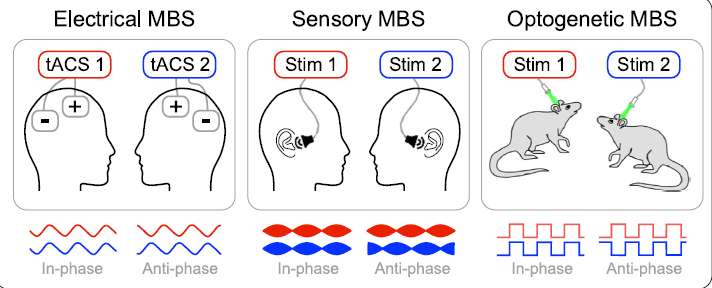
\includegraphics[scale=.70]{novembre.png} 
	\end{center} 
	\caption{\textit{Example of multi brain stimulation techniques}}
	
\end{figure}
Previous works ([Wass et al. 2020]) have been performed on humans in order to investigate the causes and effects of interbrain synchrony (often referred to as \textit{hyperscanning}). Performing an \textbf{electroencephalography (EEG)} on two interacting subjects, a strong connection has been identified between a rise in synchronization  and aspects like interpersonal coordination, cooperation and communication. In [Novembre et al. 2021], this relationship is further inspected: the simultaneous presence of synchronization and behaviour is not enough to establish a \textit{causality} between the two, which, instead, can be shown only by studying the effects which the manipulation of the first causes on the second, or viceversa. This is achieved through \textbf{multi brain stimulation (MBS)}: stimulation processes (usually of non invasive type in humans, invasive on animals) are performed on the subjects, and the provoked effects measured. Therefore, a correct analysis should combine the two approaches (hyperscanning and MBS) to be able to show true causality between interbrain synchrony and behaviour.
\\

As for interbrain analysis on mice based on microendoscopic calcium imaging, few works have been done and the topic is still largely unexplored. In one of the most significant papers, [Kingsbury et al. 2019], intracellular calcium has been recorded from neurons of the mPFC in two subjects interacting in an open arena.  The mean activity (as $\frac{\Delta F }{F}$ ) has been computed for every mouse, and the correlation between the two corresponding signals has been computed as well (using mostly cross-correlation, see Chapter 2). The first result was that animals engaged in social interaction showed higher interbrain synchronization, reporting higher values of correlation during social interaction rather than solitary periods. Moreover, the abolishment of physical interaction, using a barrier, resulted as well in the inhibition of interbrain correlation, meaning that the synchronization is not due to environmental factors, but instead strictly related to the direct interaction between conspecifics.\\

\begin{figure}[H]
	\begin{center}
		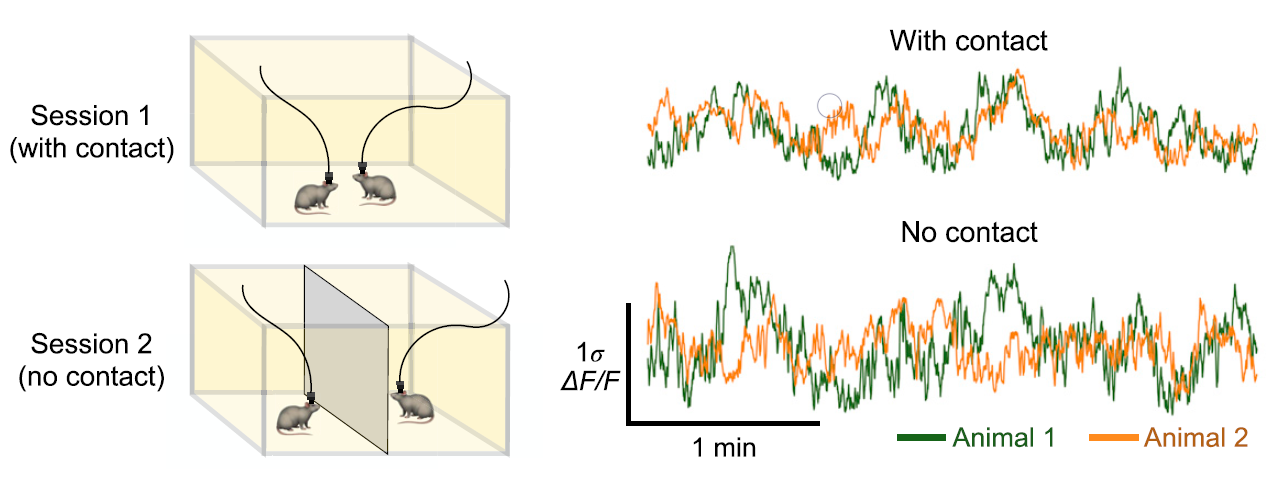
\includegraphics[scale=.70]{kingsbury.png} 
	\end{center} 
	\caption{\textit{Comparison of neuronal activities in the two mice with and without contact}}
	
\end{figure}


The second task performed in the experiment was the \textit{tube test}, in which the two subjects were placed facing each other in a horizontal tube, allowing the passage of only one individual. In this configuration, the mice can assume three types of behaviors: \textit{approach, push}, and \textit{retreat}; here animals showed again synchronization during the competitive encounters. In particular, a classification of neurons as behavioral cells allowed to link subgroups of neurons with the three types of behaviors depending on their activity values. Interestingly, the removal of these behaviour cells resulted in a marked reduction of the correlated activity. Finally, between the two animals, it was evident that one would tend to assume the role of \textit{dominant} (prevalence of push behaviour), while the other of \textit{subordinate} (prevalence of retreat). Through generalized linear models (GLMs), it has been proposed a description of the dependence between the behaviour of one mouse and the neural activity of the other, observing that cells in subordinates responded more to the ones of the dominant than vice-versa. The consequence at synchronization level is that the dominant dictates the \textit{rhythm} for the subordinate's signal, making it able to predict the expected behaviour of one mouse based on the activity of the other.







\begin{figure}[H]
	\begin{minipage}{\linewidth}
		\centering
		\begin{minipage}{0.4\linewidth}
			\begin{figure}[H]
				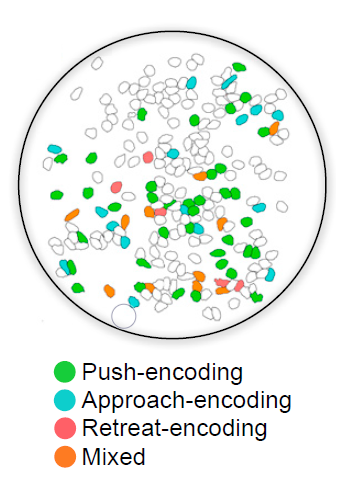
\includegraphics[width=\linewidth]{kingsbury2.png}
				
			\end{figure}
		\end{minipage}
		\hspace{0.05\linewidth}
		\begin{minipage}{0.5\linewidth}
			\begin{figure}[H]
				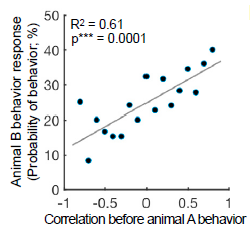
\includegraphics[width=\linewidth]{kingsbury3.png}
				
			\end{figure}
		\end{minipage}
		
	\end{minipage}
	\caption{\textit{Left: identification of behavioural neurons in the ROI. \\
			Right: correlation between the interbrain synchronization preceding behaviour in one animal and the response probability of the interacting partner}}
\end{figure}

\newpage



\section{Main tools for synchronization analysis}

In this chapter, the main tools for the analysis of synchronization between signals will be presented, with a focus on their mathematical definition and their role in the application of \textit{Intebrain synchronization}.\\
After dealing with the problem of \textit{what} synchronization actually means in this context and which measures \textit{should not} be considered, several valid tools will be proposed:\textbf{ cross-correlation}, \textbf{peak-synchronization}, \textbf{angular similarity}, \textbf{$L^2$ error analysis}. Each one of these tools has a specific purpose and meaning, and they will all be considered in the analysis of this work, in order to give different shapes to the concept of synchronization and to try to study it under the largest possible perspective.\\
Finally, when observing the presence of correlation between two signals, a different (although strongly connected) question may arise: "which is the \textit{relationship} of such connection?", or, in other words, "is one signal determining the behaviour of the other?". To answer such questions, a sophisticated tool will be object of study: the \textbf{Granger causality}.


\subsection{Understanding synchronization}

\begin{figure}[H]
	\begin{center}
		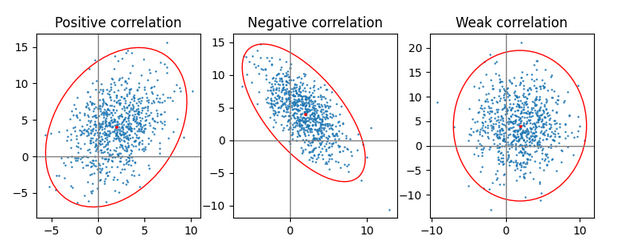
\includegraphics[scale=.75]{pearson.png} 
	\end{center} 
	\caption{\textit{Geometrical interpretation of the Pearson correlation: such coefficient gives a measure of how well the pairs obtained from the two samples distribute linearly along the diagonal of an ellipse covering the scatterplot. }}
	
\end{figure}

One of the main goals of this work will be to perform a data analysis on the Interbrain synchronization of neural signals, recorded in behavioural tasks. In order to do so, first one has to clarify the meaning of the term  \textit{synchronization}.\\
In a statistical sense, the synchronization between two time series can be seen as a measure of the \textbf{correlation} between them: the more two series are correlated, the more similar and connected they will be. This leads inevitably to the fact that, when talking about synchronization, the definition can't be unique, since the similarity between two series can be assumed in different ways, depending on the particular aspect of interest. \\
However, a first hint about what to look for or not can be found in the type of signal which is under analysis. In the present case, dealing with single neuron measurements of the intracellular concentration of $[Ca^{2+}]$ means dealing with \textit{strongly nonlinear and unstable signals}, which exhibit sudden peaks and anre often chaotic and difficult to predict.\\
For this reason, the most commonly adopted measure of correlation, namely the \textbf{Pearson correlation}, is not suited to describe such signals. Given two random samples $ \textbf{x} = \{x_i\}_{i=1}^N$ and  $ \textbf{y} = \{y_i\}_{i=1}^N$, the Pearson correlation (PC) between  $ \textbf{x}$ and  $ \textbf{y}$ is defined as

$$ \rho(x,y) = \frac{Cov(x,y)}{\sigma_x \sigma_y} = \frac{\sum_{i=1}^{N}(x_i-\bar{x}) (y_i-\bar{y})} {\sum_{i=1}^{N}(x_i-\bar{x})^2 \sum_{i=1}^{N} (y_i-\bar{y})^2} $$

where:
\begin{itemize}
	\item $ \bar{x} = \frac{1}{N}\sum_{i=1}^{N}x_i$ is the sample mean
	
	\item $Cov(x,y) = \frac{1}{N}\sum_{i=1}^{N}(x_i-\bar{x}) (y_i-\bar{y})$ is the sample covariance
	
	\item $\sigma_x = \sqrt{\frac{1}{N}\sum_{i=1}^{N}(x_i-\bar{x})^2}$ is the sample standard deviation
\end{itemize}

The PC measures the \textit{linear correlation} between two variables. This implies that this type of correlation should be used to inspect a linear relationship between two variables, which have a distribution close to the Gaussian one, and a uniform variance (i.e. reduced presence of outliers) [Applied multivariate statistics book by Johnson]. Unfortunately, with the type of data incoming from the neural recordings, all these hypoteses fail, and it follows that other correlation measures should be inspected instead.


\subsection{Cross-correlation}

When investigating the similarity between two time-dependent signals, the first tool to be considered is the \textbf{cross-correlation}.\\
Formally, given two functions $ f = f(t)$ and $ g = g(t)$, we define the cross-correlation between them as

\begin{equation}
[f(t) \star g(t)] (\tau) = \int_{-\infty}^{+\infty} f(\tau)g(t+\tau) dt 
\end{equation}


Given that the \textbf{convolution} between such functions is defined as 
\begin{equation}
[f(t) * g (t)](t) = \int_{-\infty}^{+\infty} f(t) g (t-\tau) d\tau
\end{equation}

it follows that
\begin{equation}
[f(t) \star g(t)](t) = [f(-t) * g (t)](t) 
\end{equation}

This means that the cross-correlation coincides with a convolution in which one function is considered backward in time. Moreover, in the common form of cross-correlation, as shown in (eq.1), the resulting quantity is not expressed as a function of the time variable $t$, but as a function of $\tau$, i.e. the \textit{lag} or \textit{delay} between the signals. The interpretation is straightforward: when, for a given value of the delay $\tau$, simultaneous peaks of the two signals are both present, the contribution of their product in the integral will be more relevant for the computed value of cross-correlation correspondent to  that specific lag.\\
As a consequence of this, once computing the cross-correlation between two time-dependent functions, one can identify its maximum value and retrieve the corresponding value of the lag $\tau$, from which it is possible to obtain an estimation of the delay between the two functions. To summarize, a cross-correlation analysis allows to:
\begin{enumerate}
	\item Compute the cross-correlation between the two signals as a function of the lag value  $\tau$
	
	\item Estimate the real delay between such signals, observing when the peak of cross-correlation occurs
\end{enumerate}

When the cross-correlation is computed between the same function, it takes the name of \textbf{autocorrelation}. Confronting two identical signals, there will always be a peak of correlation (equal to $1$ using \textit{normalized} cross-correlation) corresponding to the lag $\tau = 0$. Moreover, the shape of the cross-correlation will be always symmetrical (see Figure).

\begin{figure}[H]
	\begin{center}
		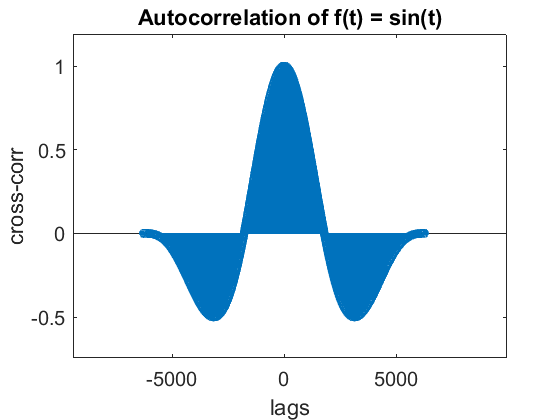
\includegraphics[scale=.75]{autocorr.png} 
	\end{center} 
	\caption{\textit{Aurocorrelation of the function $ f(t) = \sin(t) $}}
	
\end{figure}


While the autocorrelation represents an ideal case, when dealing with two different functions $f(t)$ and $g(t)$, the significance of their cross-correlation will be given by the amount of shared properties to the case of autocorrelation; however, depending on the current application, it can be reasonable to expect a peak value in correspondence to a nonzero value of the lag, as a representation of an actual physical delay.
\\

Given two time series $ \textbf{x} = \{x_i\}_{i=1}^N$ and  $\textbf{y} = \{y_i\}_{i=1}^N$, the discrete approximation of (eq.1) reads:


$$ [\textbf{x} \star \textbf{y}] (m) =  \sum_{n=1}^{N-1} x_n y_{n+m} \hspace{2cm} m_{min} < m < m_{max} $$

where $m$ is the approximate lag value, chosen in an appropriate interval.



\subsection{Peak-synchronization}

Cross-correlation is a general and widely used tool to quantify the similarity between two signals evolving in time. With the following concept of \textbf{peak-synchronization}, the focus of the analysis is restricted to the characteristic type of signal of this work: recording of intracellular calcium activity.\\
As shown in Chapter 1, a typical recording of the activity of a single neuron is characterized by the presence of rapid and intense \textit{peaks}, which define the neuron as \textit{active}. It follows that a way to intend synchronization between neurons could be related to the presence of \textit{close} or \textit{simultaneous} peaks observed at the same time. In other words, two signals (hence, neurons) are synchronized, under the peak-synchronization point of view, if a \textit{pattern} of simultaneous firing occurs. 
\\

In order to quantify the peak-synchronization between two signals, the following steps have to be faced:

\begin{figure}[H]
	\begin{center}
		\hspace*{-3cm}
		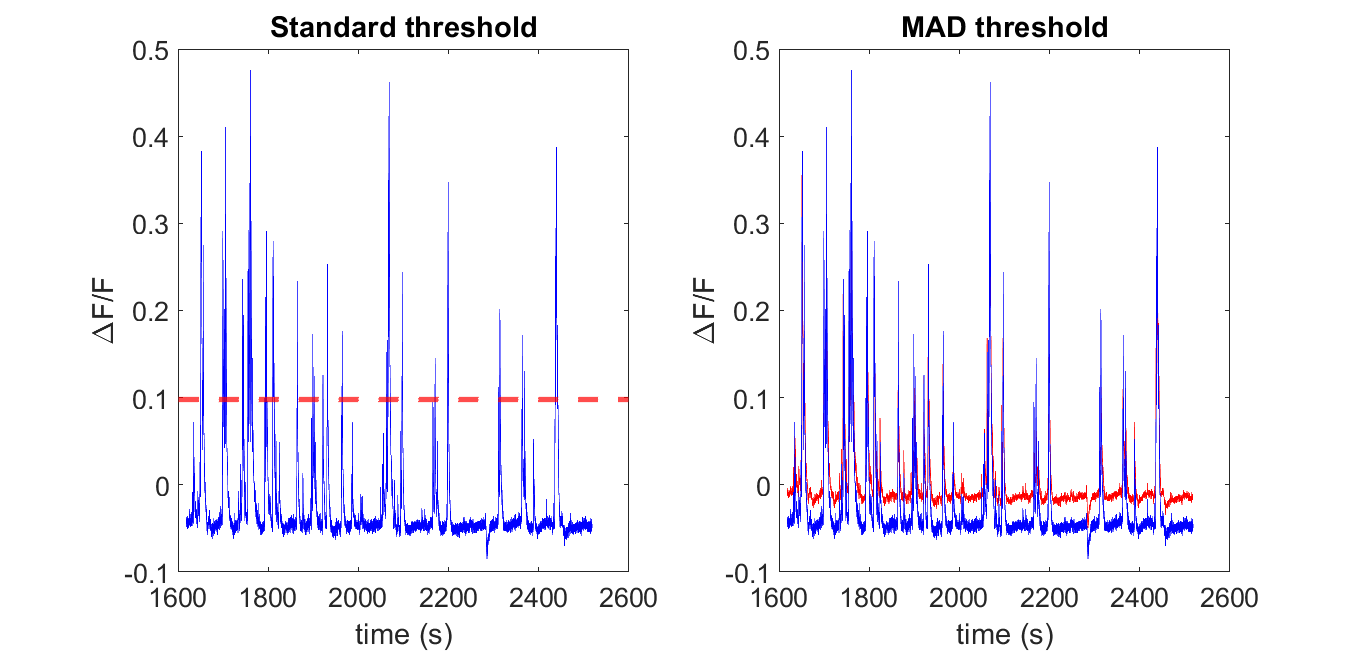
\includegraphics[scale=.50]{thresholds.png} 
	\end{center} 
	\caption{\textit{Example of a calcium signal (blue). The red curves are the thresholds built from the two algorithms: standard threshold (left panel) and MAD threshold (right panel)}}
	
\end{figure}

\begin{enumerate}
	
	\item Identify when a neuron is \textit{active}, i.e. when we are in presence of a peak
	
	\item Choose an appropriate time interval in which two neurons firing simultaneously can be considered as synchronized
	
	\item Quantify the correlation between the two neurons
	
\end{enumerate}



The way to solve all of these three steps is not unique, but it is strictly depending on the current biological application under study and by the choice of appropriate algorithms for the activity detection and  synchronization quantification. In this work, the following considerations and choices have been made:




\begin{enumerate}
	
	\item  Given a discrete time series, several algorithms are available or could be designed to detect, when a peak is occurring. A straightforward idea is to establish a threshold for the activity, in such a way that all the points above the treshold are active and all the ones below non active. Therefore, the output of such algorithm is of binary type ($1$ for activity, $0$ for non-activity).\\
	
	A naive way to define the threshold could be to consider a horizontal line, for example given by the equation $ y = \mu + 2\sigma $,	where $\mu$ and $\sigma$ are the mean and the standard deviation of the signal. In this way, all the values higher than $y$ will be considered active and vice versa. This approach is good enough when dealing with "well-behaving" signals, presenting a baseline low activity alternated by huge peaks, however it seems to fail when dealing with more complex and noisy signals.\\
	\begin{algorithm}
		\caption{Standard threshold algorithm}\label{tresh}
		\begin{algorithmic}[1]
			
			
			\State Consider a horizontal threshold given by $ y = \mu + 2\sigma $
			
			\State Confront every point of the signal with each corresponding point of the threshold
			
			\State Every point above the threshold is labeled as $1$, all the points below as $0$
		\end{algorithmic}
	\end{algorithm}
	
	
	For this reason, a different algorithm can be considered as well [Inscopix manual]: the \textbf{MAD threshold} algorithm. The threshold established by this algorithm is not constant, but it "follows" the signal, in order to better capture its dynamics. 
	
	
	
	
	
	
	
	\begin{algorithm}
		\caption{MAD threshold algorithm}\label{mad}
		\begin{algorithmic}[1]
			
			
			\State Start from a baseline threshold given by $ MAD = median(X_i - median(X))$
			
			\State Identify the points where the slope changes from positive to negative (PN) and from negative to positive (NP)
			
			
			\State At every PN point, the threshold value is the MAD value plus the previous NP point's value
			
			\State The overall threshold is obtained from linear interpolation of the threshold points
			
			\State Every point above the threshold is labeled as $1$, all the points below as $0$
		\end{algorithmic}
	\end{algorithm}
	
	\item A typical time interval in which neuronal firing occurs usually strongly depends on the specific case. However, in general it is safe to say that the peak of a neuron usually has a duration of $250-750$ ms. Such value will define the reference time window. 
	
	\item Finally, once the binary vectors of activations are available, as well as a reference time window, to quantify their synchronization, a common tool adopted is the \textbf{Peak-correlation index} [Cutts and Eglen], defined as 
	
	$$ i_{AB} = \frac{N_{AB} T}{2 N_A N_B dT} $$ 
	Here $T $ is the overall signal time window, $dT$ is the synchronization time window, $N_A$ is the number of peaks in signal A, $N_B $ is the number of peaks in signal B and finally $N_{AB} = \sum_{i=1}^{N_A} \sum_{j=1}^{N_B} I_{[-dT,dT]}(|a_i - b_j|) $ is the sum of simultaneous peaks within each synchronization window.
	
\end{enumerate}

The peak correlation index gives a representation of how well two signals (neurons) are peak-synchronized. However, it should be noticed that such measure is not normalized, meaning that the value of one index considered by itself has no real meaning, and this measure should be used only as tool to compare the same pair of signals through different phases.


\subsection{Angular distance and $L^2$ distance}

\begin{figure}[H]
	\begin{center}
		\hspace*{-3.5cm}
		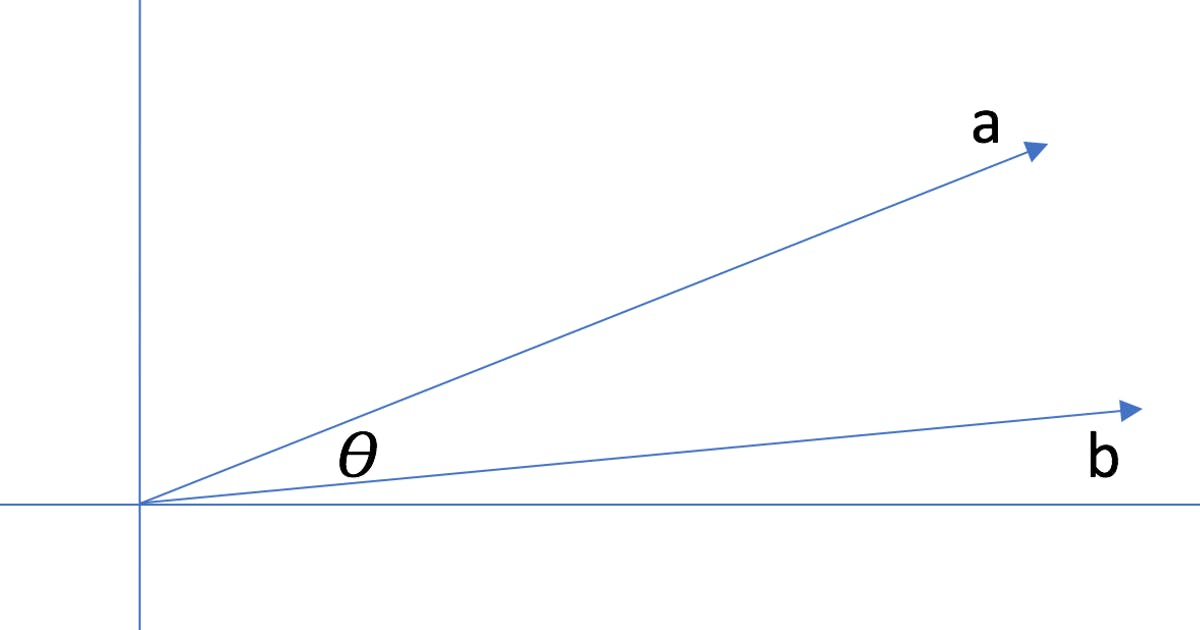
\includegraphics[scale=.20]{cos_sim.jpg} 
	\end{center} 
	\caption{\textit{Angle between two vectors in the euclidean space (2D case)}}
	
\end{figure}

Besides the two main tools for the synchronization analysis, cross-correlation and peak-synchronization, other concepts of correlation and similarity can be investigated as well. Here, two supplementary measures are considered: the \textbf{angular distance} and the \textbf{$L^2$ distance}.
\\

The purpose of the angular distance analysis is to determine the similarity between two signals in a \textit{geometric sense}. The idea is indeed rather simple: project the signals on a euclidean space and determine the angle between them. The two signals are closer, and thus more similar, if the angle between them is small.
A way to determine the angle $\theta$ between two vectors is to compute first the \textbf{cosine similarity}

$$ Sim_C(\textbf{x},\textbf{y}) = \cos \theta =  \frac{\textbf{x} \cdot \textbf{y}}{||\textbf{x}||_E ||\textbf{y}||_E} $$

where $\textbf{x} \cdot \textbf{y}$ denotes the scalar product between $\textbf{x}$ and $\textbf{y}$ and $ ||\cdot||_E$ denotes the euclidean norm.

Then, the cosine of the angle, the angular distance can be retrieved as

$$ d_\theta (\textbf{x},\textbf{y}) = \frac{\arccos(Sim_C(\textbf{x},\textbf{y}))}{\pi} $$

Where the actual angle is divided by a reference $\pi$ angle.
\\
As for the $L^2$ error, between two continuous in time signals $f = f(t)$ and $g = g(t)$ defined on an interval $[t_1,t_2]$, the $L^2$ distance between them is defined as 

$$ ||f-g||_2 = \int_{t_1}^{t_2}|f(t) - g(t)|^2 dt $$

When dealing with time discrete signals $ \textbf{x} = \{x_i\}_{i=1}^N$ and  $\textbf{y} = \{y_i\}_{i=1}^N$, this quantity it actually coincides with the \textbf{mean squared error (MSE)}

$$ MSE(\textbf{x},\textbf{y}) = \frac{1}{N}\sum_{i=1}^{N}|x_i-y_i|^2 $$


The MSE analysis performs a point-by-point comparison of the two signals, penalizing quadratically the differences between the two. It follows that in order to have a realistic estimate of this quantity, it is necessary to confront well-aligned signals. To this purpose, as described in Section 2.2, a cross-correlation analysis can be helpful, since it allows to identify the \textit{delay} between two time series, detected in correspondence of the cross-correlation peak. In conclusion, an alignment based on such value of lag between the two time signals should be performed before computing the $L^2$ distance.



\subsection{Granger causality}


\begin{figure}[H]
	\begin{center}
		\hspace*{-1cm}
		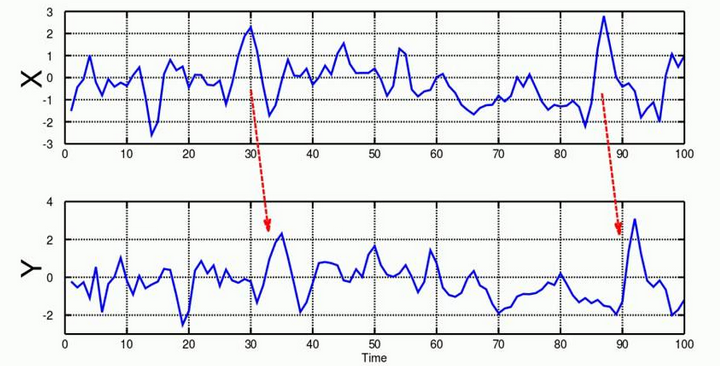
\includegraphics[scale=.60]{GC.png} 
	\end{center} 
	\caption{\textit{Example of signal X Granger-predicting signal Y }}
	
\end{figure}

As already mentioned in Section 1.5, observing a correlation between two time series 
is not enough to establish a \textit{relationship} between them. Indeed,a further indicator of  the synchronization between signals is the presence of an underlying \textit{cause-effect} mechanism underlying it all. If such relationship is found, besides observing a synchronization, one can determine also which signal (and, in this case, mouse) is responsible for causing the opponent's one.\\
In situations like the EEG experiment in [Novembre et al.] discussed in Chapter 1, such relationshipis investigated through a manipulations on the experimental level (via \textit{Multi-brain stimulation}). In  the current work, once dealing with data already measured, a different and sophisticated approach is adopted,based on statistical principles: the \textbf{Granger causality}.\\
The Granger causality (\textbf{G-causality}) is a method aimed to identify causal relationship between time series data. The word "casuality" is mainly due to historical reasons, since many debates about its correctness are still ongoing, and it would be probably more precise to refer to it as "Granger \textit{prediction}".
\\

Given two time series $ \textbf{x} = \{x_i\}_{i=1}^N$ and  $\textbf{y} = \{y_i\}_{i=1}^N$, the G-causality method is based on the following scheme:

\begin{enumerate}
	
	\item Generation of a \textbf{vector autoregression model (VAR)} of order $p$, where $p\ge 1$ is an integer to be determined, for one of the two time series, considering its previous values
	
	\begin{equation}
	\hat{x}_t = a_0 + a_1 x_{t-1} + a_2 x_{t-2} + \dots + a_p x_{t-p}
	\end{equation}
	
	
	\item Generation of a second model, in which the values of the second series are added  to  model (4)
	\begin{equation}
	\hat{x}_t = a_0 + a_1 x_{t-1} + a_2 x_{t-2} + \dots + a_p x_{t-p} + b_1 y_{t-1} + \dots + b_p y_{t-p}
	\end{equation}
	
	
	\item Comparison between the two models: if model 2 is more significant  than model 1 (in a way to be clarified in the following), then signal $\textbf{y}$ \textit{Granger-predicts} signal \textbf{x} 
	
\end{enumerate}

More formally [Barnett-Seth], given two stochastic processes $ \textbf{X} = {X}_{i=1}^N $ and $ \textbf{Y} = {Y}_{i=1}^N $, process Y \textit{does not} G-cause process X if X, conditional its past, is independent by the past of Y. A vector autoregressive model for a process $U$ takes the form

\begin{equation}
\textbf{U}_t = \sum_{k=1}^{p} A_k \textbf{U}_{t-k} + \varepsilon_t 
\end{equation}



where $p$ is the \textbf{order} of the model, $\{ A_k\}{k=1}^p$ are the \textbf{regression coefficients} and $\varepsilon_t$ the \textbf{residuals}, assumed normally and independently distributed. The \textbf{ residual covariance matrix} of the model is defined as $ \Sigma = Cov(\varepsilon_t) $ and it is assumed to be stationary. The process $U$ can then be identified both as $X$ and $Y$. Given a VAR model of the form (6), the \textbf{autocovariance sequence} $ \{\Gamma_k\}_{k=1}^p $ is defined as $ \Gamma_k = Cov(\textbf{U}_t,\textbf{U}_{t-k})$, and it is possible to relate this quantity to the autoregression coefficients $\{ A_k\}$ thanks to the \textbf{Yule-Walker} equations [Anderson,1971]

\begin{equation}
\Gamma_k = \sum_{i=1}^{p} A_i \Gamma_{k-i} + \delta \Sigma \hspace{1 cm }  k = 1, \cdots, p
\end{equation}\\

Standard VAR theory [Hamilton-Lutkephol] requires the condition $ \sum_{k=1}^{N}||A_k||^2 < \infty $. Moreover, defining the \textbf{characteristic polynomial} as 
$$ \phi_A(z)= \det \left( I - \sum_{k=1}^{p} A_k z^k \right) $$
it must be that the \textbf{spectral radius} $\rho(A) := \max_{\phi_A(z)=0}|z|^{-1}$ is strictly less than $1$, as a \textit{stability} condition.
\\

Considering now a process in which $ \textbf{U}_t = \begin{bmatrix} \textbf{X}_t  \\  \textbf{Y}_t \end{bmatrix} $, its VAR formulation reads

\begin{equation}
\textbf{U}_t = \sum_{k=1}^{p} \begin{bmatrix} A_{xx,k}  &  A_{xy,k} \\  A_{yx,k}  & A_{yy,k} \end{bmatrix} \textbf{U}_{t-k} + \begin{bmatrix} \varepsilon_{x,t}  \\  \varepsilon_{y,t} \end{bmatrix}
\end{equation}


and its residual covariance is $ \Sigma = Cov\left(\begin{bmatrix} \varepsilon_{x,t}  \\  \varepsilon_{y,t} \end{bmatrix}\right) = \begin{bmatrix} \Sigma_{xx}  &  \Sigma_{xy} \\  \Sigma_{yx}  & \Sigma_{yy} \end{bmatrix} $.\\
This augmented formulation contains both the regression models for process $X$ and $Y$. For example, its first component reads

\begin{equation}
\textbf{X}_t = \sum_{k=1}^{p} A_{xx,k} \textbf{X}_{t-k} + \sum_{k=1}^{p} A_{xy,k}  \textbf{Y}_{t-k} + \varepsilon_{x,t}
\end{equation}

If the process $Y$ does not G-cause the process $X$, it follows that the coefficients $\{A_{xy,k}\}_{k=1}^p $ are all equal to $0$, and the model becomes

\begin{equation}
\textbf{X}_t = \sum_{k=1}^{p} A'_{xx,k} \textbf{X}_{t-k} + \varepsilon'_{x,t}
\end{equation}

Therefore, a statistic test checking  the null hypothesis \{$ H_0:  Y \hspace{0.2cm} \text{does not G-predicts} \hspace{0.2 cm} X $\} has the form

\begin{equation}
H_0: A_{xy,1} = A_{xy,2} = \cdots = A_{xy,p} = 0
\end{equation}


If  $\Sigma'_{xx} = Cov(\varepsilon'_{x,t}) $ is the residual covariance matrix of model (10), standard theory [Edwards, 1992] suggests the use of the \textbf{(log-)likelihood statistics} to obtain a \textit{maximum-likelihood} estimator of the G-causality between $Y$ and $X$ (here referred as $ \mathcal{F}_{Y \rightarrow X} $):

\begin{equation}
\mathcal{F}_{Y \rightarrow X}  = \ln \frac{det(\Sigma'_{xx})}{det(\Sigma_{xx})}
\end{equation}


Since the determinant of a covariance matrix (i.e. the \textit{generalized variance}) quantifies the \textit{prediction error} of its regression model, the interpretation of (11) is that the G-causality statistics  $ \mathcal{F}_{Y \rightarrow X} $ is a measure of how much the prediction error is reduced when also the process $Y$ is included in the regression model. Clearly, this same procedure applies to the statistics  $ \mathcal{F}_{X \rightarrow Y} $, in which the directionality of the relationship is inverted. It can be proven [Wilks \& Wald] that, under the null hypothesis, $ (N-p)\mathcal{F}_{Y \rightarrow X} \sim \chi^2(d)$, where $ d = pN^2$.
\\
To summarize, the typical workflow for G-causality estimation, consists in the following steps:

\begin{enumerate}
	\item Estimate the model order $p$ via appropriate criterion (such as AIC and BIC)
	
	\item Estimate the autocovariance sequence $\Gamma_k$ and the VAR coefficients $(A_k, \Sigma)$ through the Yule-Walker equations (7), both for reduced and augmented models. Verify that $ \sum_{k=1}^{N}||A_k||^2 < \infty $ and  $\rho(A) < 1$
	
	\item Computation of the G-statistics $ \mathcal{F}_{Y \rightarrow X} $ and $ \mathcal{F}_{X \rightarrow Y} $ through (12)
	
	\item Test the significance of the statistical tests against the null hypotesis, computing the $p$ -values of the two tests 
	
\end{enumerate}

\newpage
\section{Interbrain data analysis: one-to-one task}





\newpage
\section{Interbrain data analysis: emotion discrimination task}

In this second chapter, the main results on the data analysis on the emotion discrimination task are presented. After describing the phases of the task and trying to understand whcih an be an appropriate way  to represent the data, through normalizations, first results on the neural activity of mice in relation to their behaviour are presented. Then, the focus goes on the main part of the analysis: the interbrain synchrony between such activities. The different concepts of synchrony introduced in Chapter 2 habe been investigated, such as the study of causality between signal via Granger prediction. 


\subsection{Emotion discrimination task}

\begin{figure}[H]
	\begin{center}
		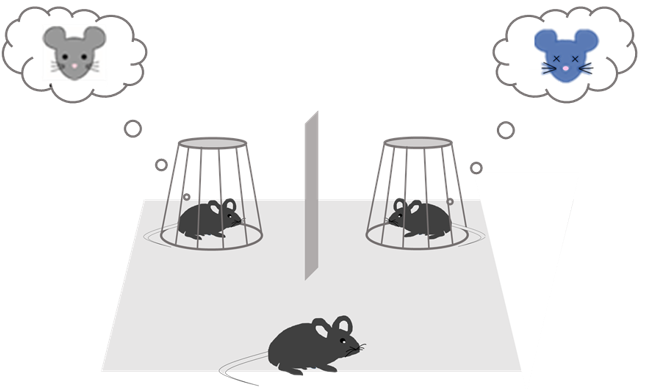
\includegraphics[scale=.90]{emotion_discrimination.png} 
	\end{center} 
	\caption{\textit{Scheme of the emotion discrimination task}}
	
\end{figure}

The \textit{emotion discrimination task} consists of an observer mouse facing two demonstrators in an open arena. One demonstrator is in a \textit{neutral} state, the other in a \textit{stressed} state, i.e. it has been subjected to a \textit{stress protocol} (forced restrainment) before the test. The task consists of three main parts:

\begin{enumerate}
	
	\item \textbf{Homecage restrainment}: the three mice are kept separate in a cage in normal conditions. \\
	$\longrightarrow$ \textit{Duration}: 5 minutes
	
	\item \textbf{Habituation}: the observer mouse is free to move in an empty open arena; in the meantime the neutral demonstrator is kept in the cage, while the stressed demonstrator is being subjected to the stressing procedure \\
	$\longrightarrow$  \textit{Duration}: 15 minutes
	
	\item \textbf{Test}: the demonstrators join the observer in the arena. Only the observer is free to move, since the two demonstrators are kept behind a cage allowing sight, sniffing but no passage \\
	$\longrightarrow$  \textit{Duration}: 15 minutes
\end{enumerate}

During all the three phases, the neural activities of the three mice are recorded via microendoscopic calcium imaging as described in Section 1.3, in which the target are \textit{somatostating-expressing} interneurons in the anterior cingulate cortex (Section 1.1). Moreover, the position of the observer mouse along time is recorded during habituation and test phases, such as TTL signals (binary recording of events) of the reciprocal sniffing between one observer and a demonstrators have been measured during the test. Finally, spatial data of the neurons in the \textit{region of interest (ROI)} captured by the miniscope, are present as well, such as their position and size.\\
These type of data can lead to several analyses:
\begin{itemize}
	
	\item Inspecting if there are correlations between the neural activity levels of one mouse and what is happening during the task, such as the stressing procedure or the proximity of two mice
	
	\item Testing the presence of \textit{activity synchronization}, as described in Section 2.1-2.4, between the neural signals of two mice, in relation to what is happening in the test (proximity of two subjects, sniffing...)
	
	\item Investigating whether the activity in one mice is \textit{predicting} the activity in another, for example via a Granger causality analysis introduced in Section 2.5
	
	\item Wondering wether the neuronal firing in single mice seems to follow \textit{patterns}, or if it is possible to predict mathematically such chain of events (problem dealt in Chapter 7)
\end{itemize}


The analyses have been conducted on 3 different datasets, meaning that 3 triplets of mice tested with the same procedure. Moreover two more experiments have been performed in the so called \textbf{self-experience} setting, in which, before the test, also the observer is subjected to a stress protocol.\\
It is worth to stress the fact that the phases of homecage and habituation play the role of a \textit{control} in the data analysis: given a quantity measured from the data of calcium concentrations, we can assume that a result is significant, and thus related to the interactions between mice, if it is present in the test phase but not in the control phases of homecage and habituation, in which the mice cannot interact and are located in different places.

\subsection{Normalizing the dataset}


\begin{figure}[H]
	
	\begin{center}
		\hspace*{-2.1cm}
		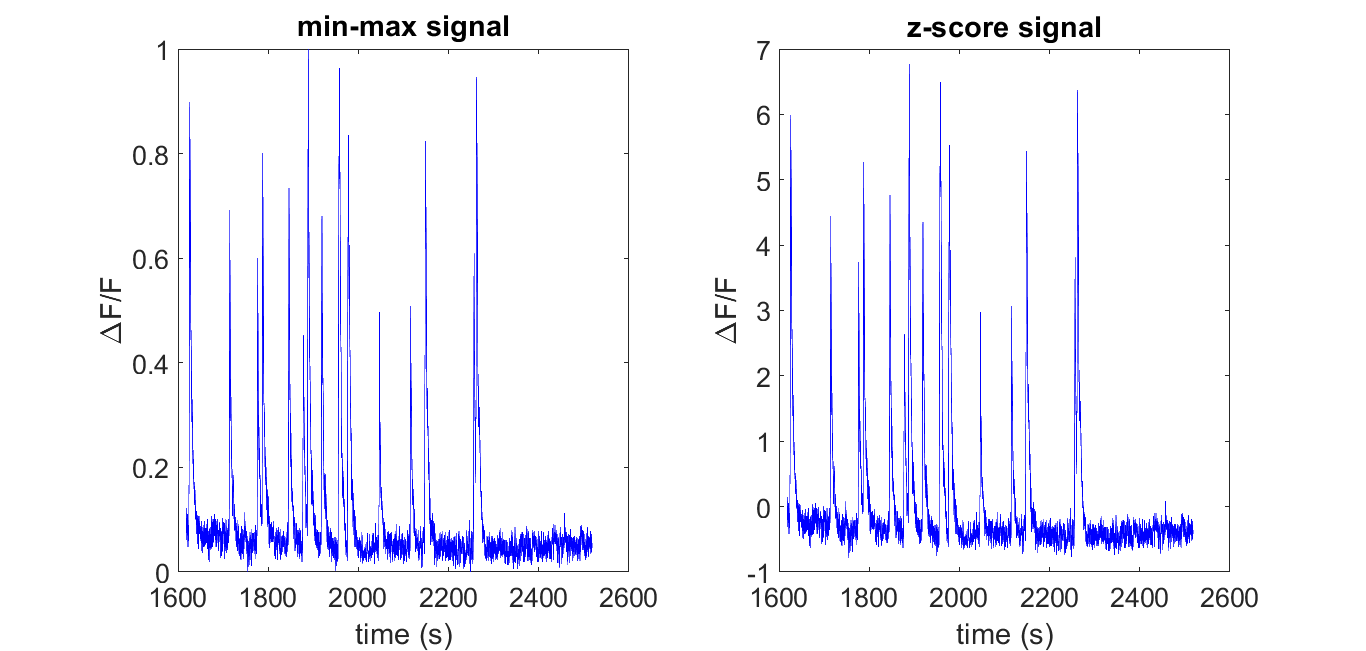
\includegraphics[scale=.45]{normalizations.png} 
	\end{center} 
	\caption{\textit{Left: min-max normalization, with signal in $[0,1]$. Right: z-score normalization, with no constrain on the scale. }}
	
\end{figure}
The main objects of the analysis are the calcium tracks recorded in every single neurons, expressed in terms of relative fluorescence $\frac{\Delta F}{F}$. Such signals will be subjected to operations (such as mean) and comparisons, both between neurons of a single mouse, and between activities of different mice. It necesessarely follows that it is fundamental to determine a priori a \textit{normalization} of the data which can allow such processes. The literature proposes several ways to threat data, for example: (see Figure):

\begin{enumerate}
	
	\item \textbf{Raw approach}. The raw data, coming from the Inscopix pre-processing described in Section 1.4, are usually not ready to be analyzed yet. Although normalizations on the videos, filtering, nose detection process have been already performed, the single information of a fluorescence value $\frac{\Delta F}{F}$ needs to be threated carefully. Every single neuron is characterized by a baseline activity, alternated with rapid and huge calcium spikes. Such baseline value, even if biiologically represents in any case a non active neuron, can have difference values across neurons. Moreover, the value reached by every spike can be quite different across different neurons, but this not necessarely reflects the same difference in what is really happening in the neuron: a spike can be less marked for the simple fact that less GCaMP protein was present at that moment, and consequently the spiking of that neuron happened at a smaller scale, preserving however its shape. 
	
	\item \textbf{min-max normalization}. With the min-max normalization, every value $x_t$ of the signal $ x = \left\{ x_t\right\}_{t=1}^N$ at time $t$ is normalized through
	
	\begin{equation}
	x_t^{mm} = \frac{x_t -  \min(x)}{\max(x) - \min(x)}
	\end{equation}
	
	With the min-max normalization, all the signals are bounded in the iterval $[0,1]$, in which the limit values are assumed by the highest and lowest values, respectively. Therefore, using this normalization, all the signals are threated in the same way, since they are all uniformed in the same interval, whatever it was their original value.
	
	\item \textbf{z-score normalization}. For a value  $x_t$ of the signal $ x = \left\{ x_t\right\}_{t=1}^N$, the z-score normalization reads
	
	\begin{equation}
	x_t^{z} = \frac{x_t -  \mu}{\sigma}
	\end{equation}
	
	where $\mu$ and $\sigma$ are the mean and standard deviation of the signal, respecitively. The goal of this normalization is to bring every signal at mean $0$ and standard deviation $1$, making them more comparable without directly putting constrains on their values, as it was in the case of the min-max normalization
	
	
\end{enumerate}


All the different normalization does not modify the shape, but they modify the \textit{scale} of the values. As for this work, the choice went on a normalization \textbf{z-score on baseline}, in which signals are aligned and then divided by their dìstandard deviations such as in the z-score case, but the alignment is not performed on their mean. The reason for this is that two signals of this type may have the same mean, but different baseline activities. Therefore, the alignment is done on such baselines, which are set to $0$ for every neuron.



\subsection{Behavioural analyses of the task}


\begin{figure}[H]
	
	%\begin{center}
	\centering
	
	\hspace*{-1.4 cm}
	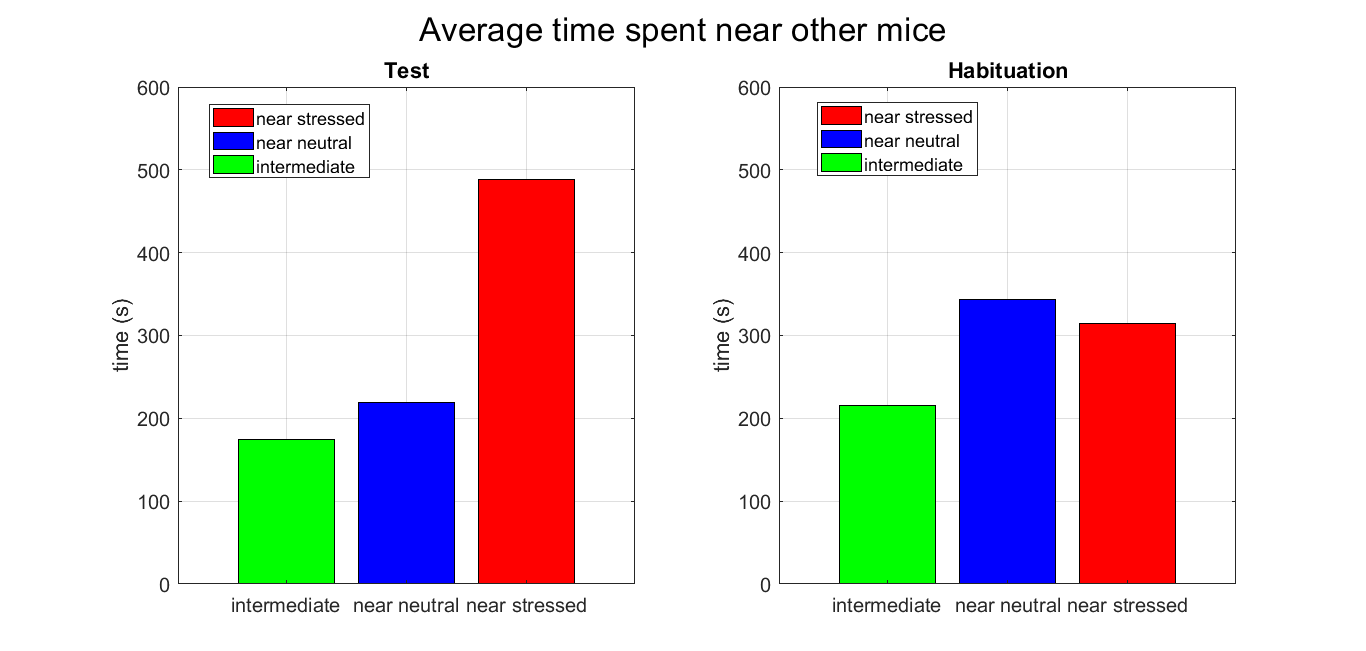
\includegraphics[scale=.42]{times.png} 
	%\end{center} 
	\caption{\textit{Average time spent by the observer near the demonstrator cages, or in the intermediate area. Left: results during the test. Right: results during the habituation. }}
	
\end{figure}

In the work of [Scheggia-Managò], the same neuronal population, namely the somatostin interneurons, had been observed during a task following a similar protocol of the current emotion discrimination task. In that case, however, the area of interest was the medial prefrontal cortex, and the main focus on the activity was in electrophyisiology. As results, it was evident that the observer mouse spent more time near the stressed demonstrators, and its neural activity (in terms of action potentials) showed higher values in those periods.\\
As for the current work, similar analyses produced the following results:

\begin{itemize}
	\item The observer spent a significantly higher time near the stressed demonstrators, rather than near the neutral one or in an intermediate zone (see Figure). Moreover, in order to rule rule that this effect was due to spatial factors present in the area in which the stressed mouse was located, a comparison with the habituation has been performed. During the habituation, the observer is free to move in the arena for the same time of the test, but in the arena the two cages for the demonstrators are empty. The results show clearly that in this situation the observer doesn't show a particular tendency for proximity, and in particular spend considerably less time near the cage of the stressed mouse.
	
	\item As for the calcium activity, no evidence of correlation seemed to emerge: from the recorded neurons, the observer mantains an overall similar average activity through the different areas of the arena. As for the demonstrators, only the neutral appears to show an increase activity during the sniffing with the observer.
	\\
	
	Next, a comparison on the average activity of mice during the phases of the task have been taken into account (see Figure). The results showed that, in general, the mean activity seems to be higher during the habituation. This happens in particular for the stressed mouse, coherently with the fact that during the habituation, it is being subjected to the stress protocol (forced restrainment), for which it is expected to show higher activity. Overall, the neutral mouse shows smaller values of calcium activity, both during habituation and test, compared to the observer and the stressed conspecifics.
	
\end{itemize}


\begin{figure}[H]
	
	\begin{center}
		\hspace*{-1.6cm}
		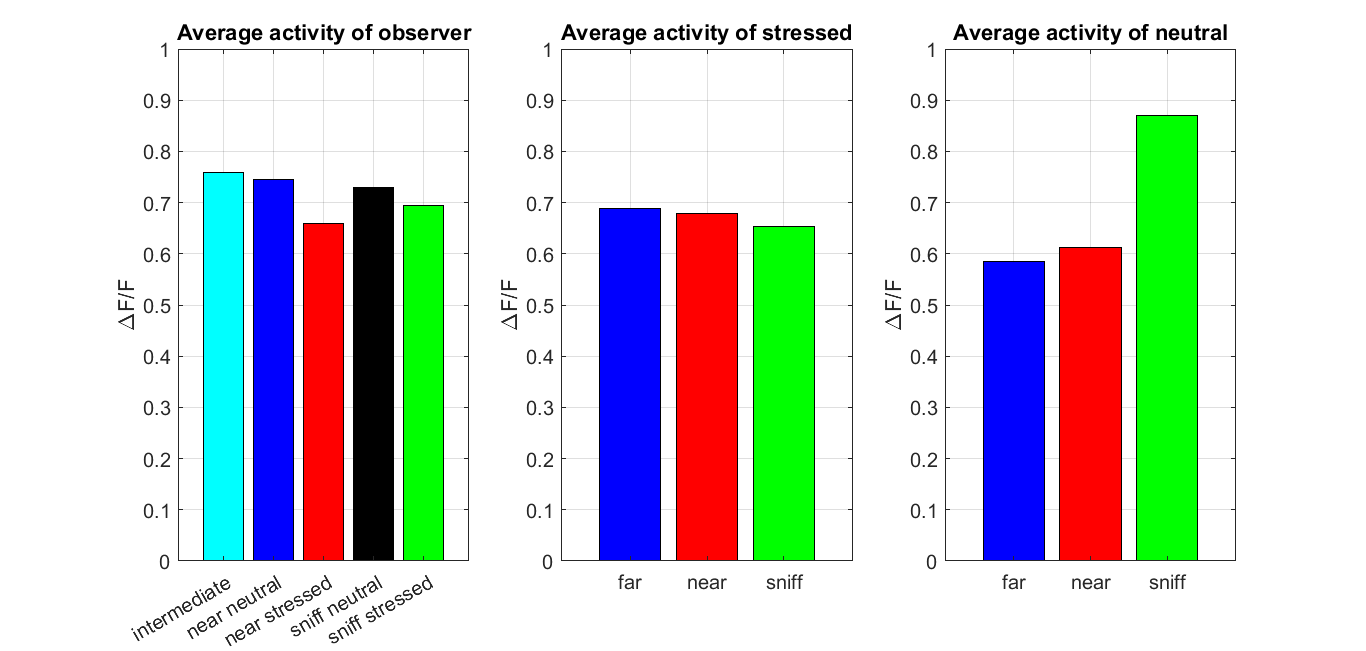
\includegraphics[scale=.42]{activity_barplot.png} 
	\end{center} 
	\caption{\textit{Average activity showed by the mice. Left: observer. No tendencies seem to emerge when it is in intermediate area, close to demonstrators or sniffing with demonstrators. Center: stressed. No tendencies seem to emerge comparing the periods when the observer is far, near or sniffing the stressed Right:neutral. During the sniffing with the observer, its activity shows higher values}}
	
\end{figure}


\begin{figure}[H]
	
	\begin{center}
		
		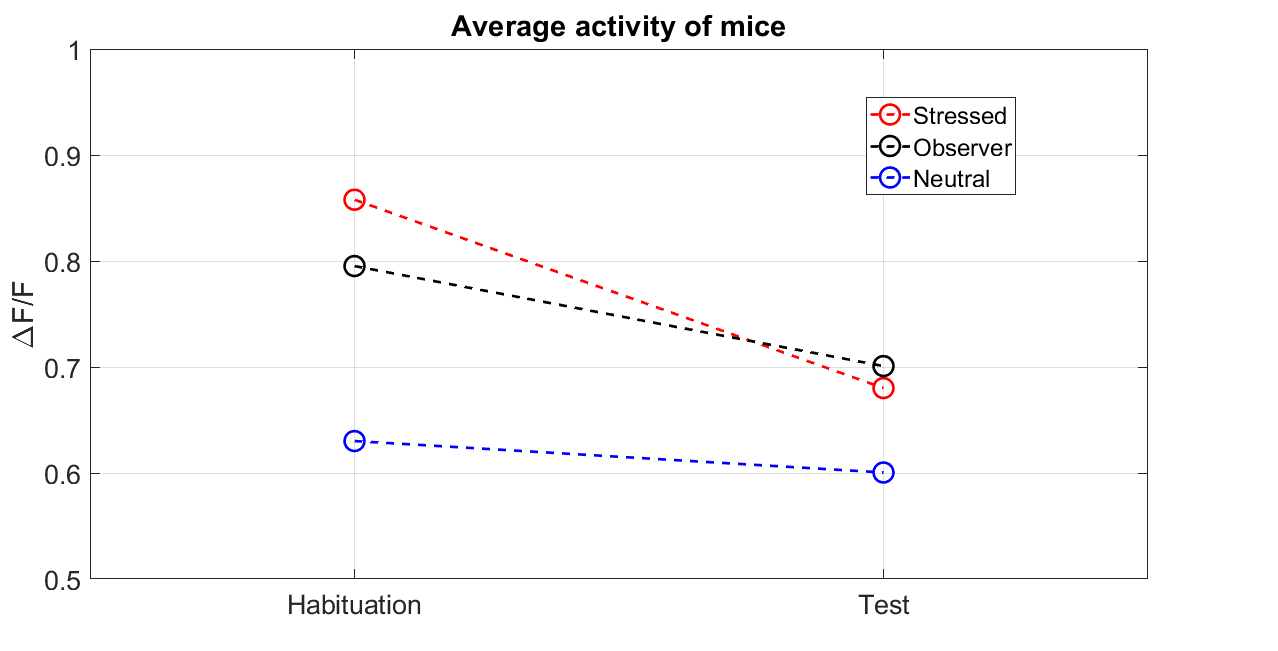
\includegraphics[scale=.4]{activities.png} 
	\end{center} 
	\caption{\textit{Evolution of the average activity of the three mice from the habituation to the test}}
	
\end{figure}


\subsection{Cross-correlation analysis for the mean activity}

\begin{figure}[H]
	
	\begin{center}
		\hspace*{-1.4cm}
		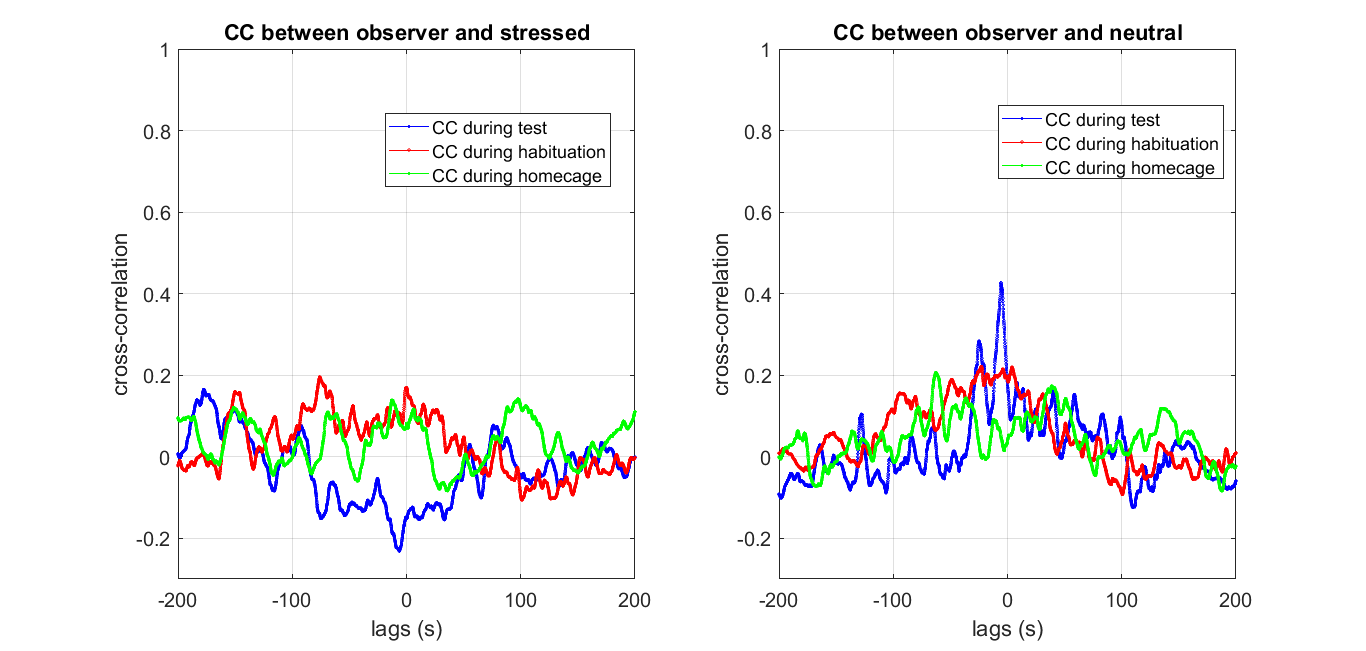
\includegraphics[scale=.4]{average_cc.png} 
	\end{center} 
	\caption{\textit{Left: average cross-correlation between observer and stressed. Right: average cross-correlation between observer and neutral}}
	
\end{figure}

With the \textit{Interbrain analysis}, we wonder whether the interactions of two mice are followed by a synchronization of their neural signals. As explained in Section 2.2, one of the main tool for the synchronization analysis is the \textbf{cross-correlation}.\\
As first step, following the approach of [Kingsbury], every mice has been gifted with its \textit{overall activity}, consisting in a mean of the activities of all its recorded neurons. Such activities can be considered in several parts:

\begin{enumerate}
	\item Restriction to the times of proximity between the observer and the stressed
	\item Restriction to the times of proximity between the observer and the neutral
	\item Restriction to the times of reciprocal sniffing between two mice
\end{enumerate}

so that we can analyze the correlation between the activities of two mice when they are actually close to each other. In this context, a cross-correlation analysis on the mean activity has been performed, comparing what happens during the homecage, habituation and test (see Figure). During homecage and habituation phases, the three mice are kept separate. Therefore, inspecting the correlation between the activites during these phases is a useful \textit{control}, i.e. a case of comparison in order to see what to expect when correlation should not be present.
\\

As first analysis, an overall activity of the inspected ROI has been considered. A mean of all the $\frac{\Delta F}{F}$ signals in each neurons has been computed for every mice, and subdivided in the parts defined by 1-3. Next, the cross correlation between observer and stressed and observer and neutral mean activies has been computed as described in (ref chap 2). As shown in Figure, analyzing the average cross correlation between the two experiments one can notice the presence of a peak around $ lag=0 $ for the pair observer-neutral in the test phase. This tendency is not present in the control cases of habituation and homecage, making it proper of the test. On the other side,the cross correlation between observer and stressed does not show any particular difference with respect to the homecage and habituation ones. A further control has been given by observing the cross correlation between the observer and one demonstrator considering the periods when the observer was visiting the other demonstrator. As result, the cross correlation between observer and neutral is abolished considering the instants when the observ was visiting the stressed, and the cross correlation between observer and stressed remains non signficative when the observer is visiting the neutral. Overall, these results may show the presence of a synchronization between neural activities between the observer and the neutral mouse, but not between the observer and the stressed, and this effect is present only during the test and during the proximity of the two mice.\\
Next, two particulr cases have been considered: the sniffing interactions and the first part (2 minutes of the test). The sniffing is known to be one of the most direct interactions that two mice can display between each other, and therefore is of a particular interest for what could happen at synchronization level. The restriction to the first two minutes of the test is of interest based on previous results [Kingsbury], which show that the first periods of interactions between mice is the one which determine the most some relevant neural tendency, such as synchronization. The results obtained showed the following (Figure):

\begin{itemize}
	\item The result during the sniffing interactions are coherent with the ones obtained during the whole test: a peak around $lag=0$ is present only in the cross corelation computed between observer and neutral, but not oberver and stressed
	
	\item In consistence with previous results, the peak of cross correlation between observer and neutral is higher if we restrict the analysis to the first two minutes of interaction. A visual confirmation of the improve in synchronization in the test rather than habituation in this case is given by Figure
	
\end{itemize}

A summary of the cross-correlation results can be see in Figure. For every case, the values refer to the cross-correlation peak recorded around $lag=0$. While for the observer-stressed case no particular difference arise, between observer and neutral the test phases show higher correlations, in particcular thr sniffing and the beginning of the test.

\begin{figure}[H]
	
	\begin{center}
		\hspace*{-1.4cm}
		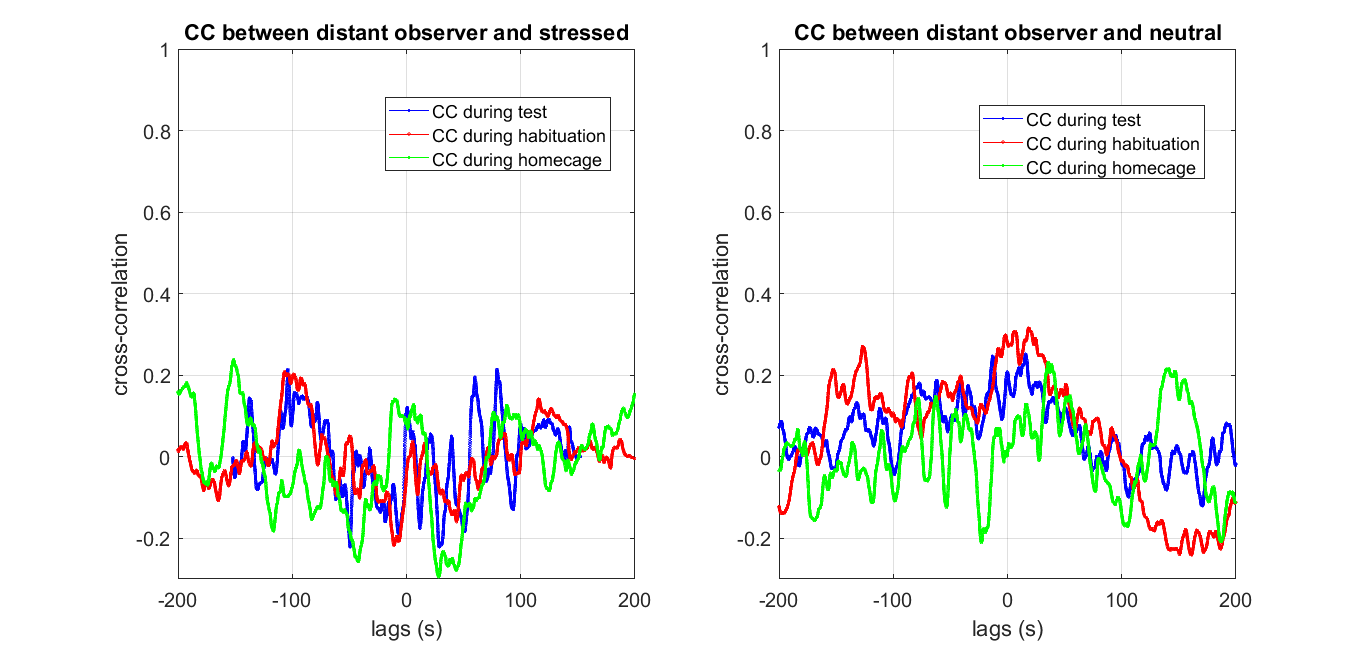
\includegraphics[scale=.4]{cc_distant.png} 
	\end{center} 
	\caption{\textit{Left: average cross-correlation peaks between observer and stressed when observer is visiting neutral. Right: average cross-correlation peaks between observer and and neutral when observer is visiting stressed.}}
	
\end{figure}

\begin{figure}[H]
	
	\begin{center}
		\hspace*{-1.4cm}
		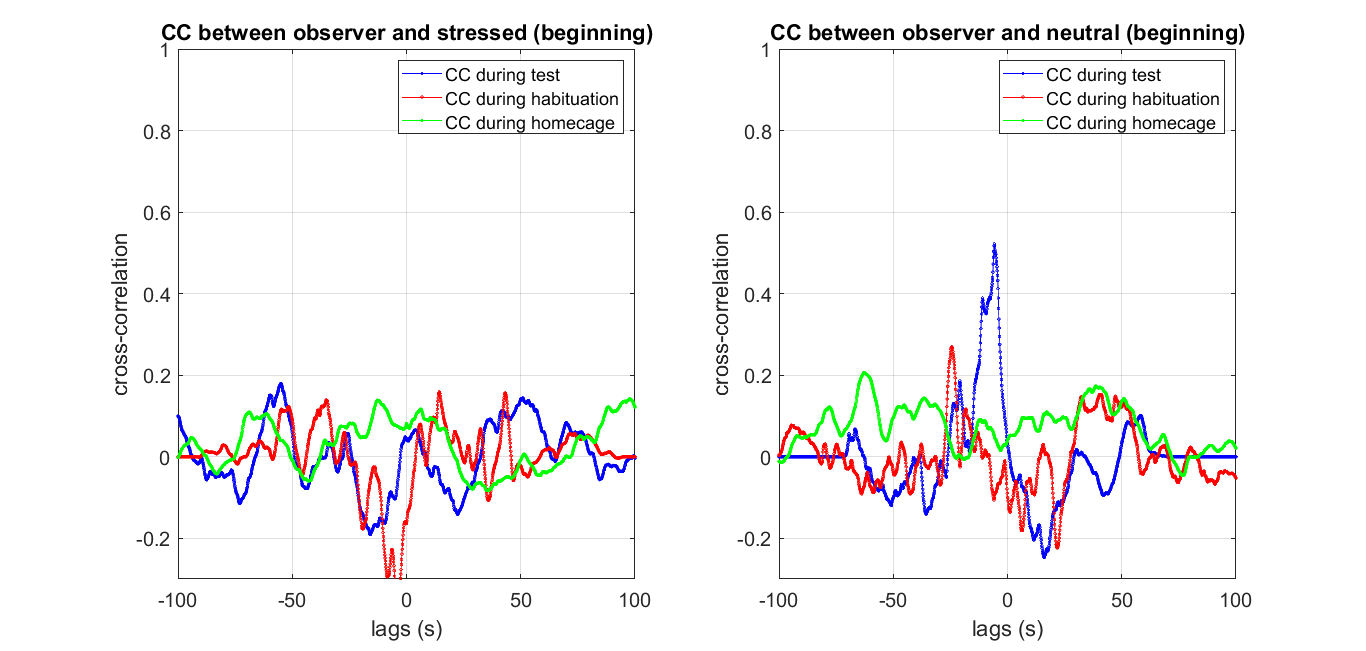
\includegraphics[scale=.4]{average_cc_initial.png} 
	\end{center} 
	\caption{\textit{Left: average cross-correlation between observer and stressed, during the first two minutes of test. Right: average cross-correlation between observer and neutral, during the first two minutes of test.}}
	
\end{figure}

\begin{figure}[H]
	
	\begin{center}
		\hspace*{-1.4cm}
		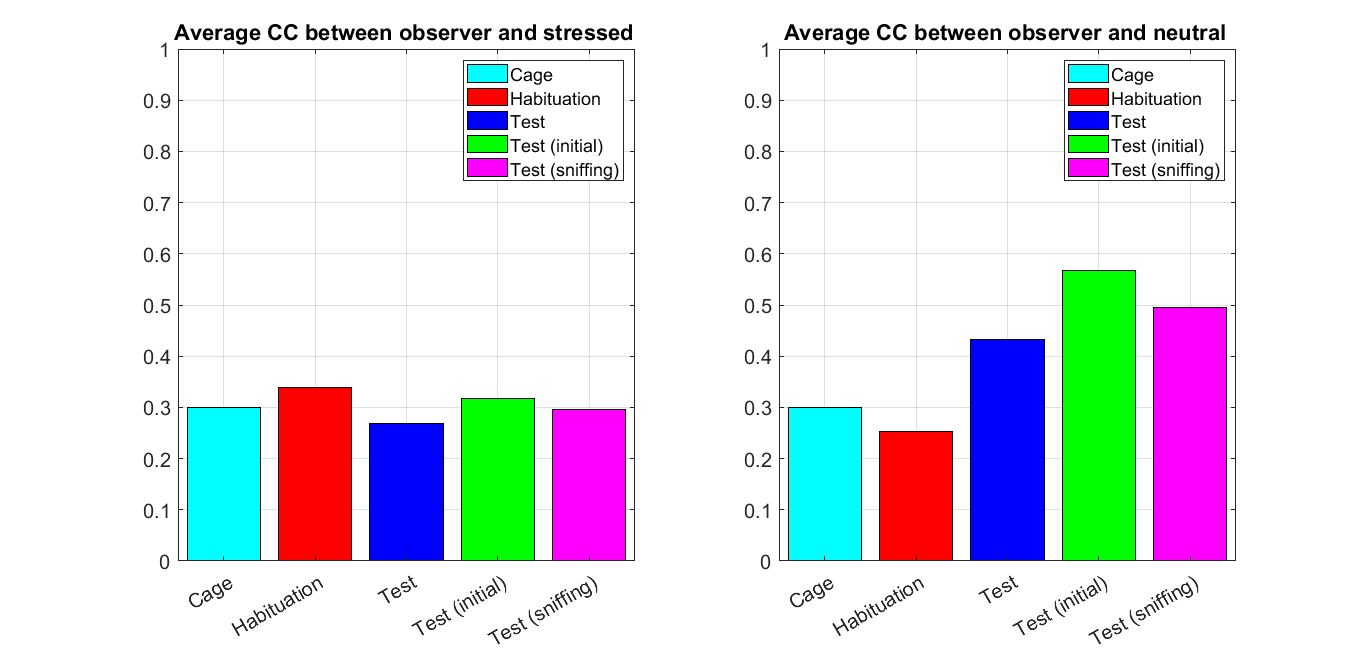
\includegraphics[scale=.4]{cc_average.png} 
	\end{center} 
	\caption{\textit{Left: average cross-correlation peaks between observer and stressed. Right: average cross-correlation peaks between observer and and neutral.}}
	
\end{figure}




\newpage
\section{Activity of amygdala in altruistic decision making}

In this chapter, a new aspect of the behavioural analysis from in vivo tasks on mice will be investigated: the ability of mice to display selfish or prosocial choices towards other individuals.\\
Through the \textit{altruism task}, two mice are put in a situation in which they can choose whether to perform an altruistic or selfish choice, while having their neural activity recorded. In this context, however, the employed technique for calcium imaging is not microendoscopic calcium imaging, but \textit{Fiberphotometry} (discussed in Section 1.4), from which an overall signal containing the calcium activity is obtained.\\
As for the area of the brain under investigation, in this case the focus is on the \textbf{basolateral amygdala (BLA)}, which has been shown to be connected with prosocial choices in rodents (Sextion 1.1).\\
After describing the results of the altruism task in terms of behaviour, the focus will concern with the analysis of the calcium tracks from fiberphotometry, and in particular their relative change with respect to a baseline activity, when making prosocial or selfish choices.


\subsection{Social decision making in mammals}

In order to live as a group, mammals have to perform decisions based on their \textit{social interactions}. Often, such decisions are strictly egoistic and selfish, in order to survive as a single individual and obtain the best for itself. However, evolution taught us that \textbf{altruistic} decisions, engaged with the purpose of creating a benefit for the entire community, are present as well, and are actually necessary in order to survive in social groups [Batson, C. D.].\\
The reasons behind whether a social choice may be of altruistic rather than selfish type are often nontrivial and may depend on several factors, such as the presence of a \textit{dominance} relation inside a group, the degree of closeness between two individuals, or biological factors like age and gender.\\
In the first years of study of social interactions and decision making, the term \textit{altruism} was used only for humans, but, along the years, the increase of discoveries of similar attributes in other animals changed the situation. For example, frequent habits of sharing food have been observed in parrots [Brucks, D. \& von Bayern] and monkeys [Krupenye, C., Tan, J. \& Hare]. Mice do not differ: rodents have been shown to display altruistic decision making such as consolatory and collaborative behaviours, or help to conspecific in case of need [Bartal, I. B.-A., Decety, J. \& Mason]. \\
Moreover, a dysfunctional behaviour in social decision making, such as a lack of empathy, could be strictly related to many psycho-pathologic conditions such as schizophrenia, autism, Alzheimer's disease or dementia. \\
Through the years, the interest in observation of social decision making in groups of mammals has been growing. However, very often the focus of such studies is limited to the \textit{expressed} behaviour, rather than the characterization of the underlying neural causes. Recently, studies on primates [Dal Monte, O., Chu, C. C. J., Fagan] seem to have identified the neural circuits responsible for social interactions and decision making in the basolateral amygdala (BLA), and following studies on mice confirmed it as well [Felix-Ortiz, A. C., Burgos-Robles, A., Bhagat].

\subsection{Description of the altruism task}

\begin{figure}[H]
	\begin{center}
		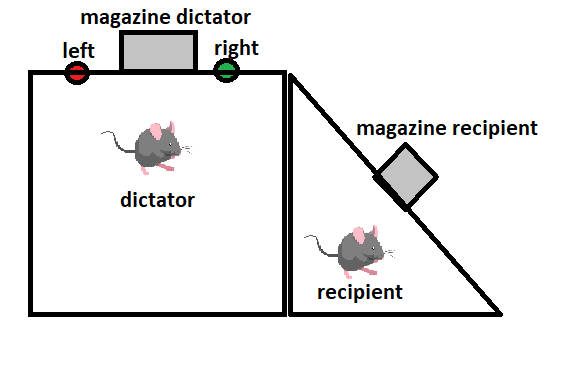
\includegraphics[scale=1.1]{altruism.png} 
	\end{center} 
	\caption{\textit{Main setting of the altruism task: a dictator mouse (left) can choose between two pokes, one of which will deliver a food pellet to a recipient mouse (right)}}
	
\end{figure}

The \textit{altruism task} is a task in which two mice are tested in their social decision making. It consists in two mice located in adjacent compartments, separated by a metal mesh which allows them to see and sniff each other, but not enter in direct contact. One mouse, called the \textit{recipient}, assumes only a passive role: it stays in its space and, when a food delivery happens from an apposite box (called \textit{magazine}) it can eat the delivered food pellet. 
In contrast, the other mouse, called \textit{dictator}, has to perform a social choice. Indeed, in any case a food delivery to its own magazine will happen by poking one of two buttons available, but even if both types of pokes will provoke a pellet delivery for the dictator, only one of them will give food to the recipient as well. It follows that the two choices of the dictator can be classified as \textit{selfish} and \textit{altruistic} decisions.\\
In order to stimulate the seeking for food, mice have been kept at $ 90 \%$ of their standard body weight before the test. The setup is organized as follows:

\begin{itemize}
	
	\item Before the tasks were performed, both mice were kept together in same sex pairs for two weeks 
	
	\item The animals were tested for $5$ days. The first day involves a \textit{learning} process for the dictator to understand the food delivery mechanism. The main test is considered to be during the following $3$ days, and finally the process is considered well assimilated by the dictator during the final day	
	
	\item The position of the altruistic and selfish pokes (i.e. of the two buttons providing or not the food delivery to the recipient) has been randomized through the different days of the test, in order to rule out spatial causes for the results
	
	\item A control test has been performed in parallel. Here, the recipient mice were replaced by inanimate objects, in order to determine the effective relevance of their presence in the task
	
	\item During the performance of the $5$ days of the test, the calcium activity in the basolateral amygdala of the dictator has been recorded using the Fiberphotometry technique, giving as result a collective signal (as discussed in Section 1.4)
	
\end{itemize}



\subsection{Behavioural results in the altruism task}


\begin{figure}[H]
	\begin{minipage}{\linewidth}
		\centering
		\begin{minipage}{0.46\linewidth}
			\begin{figure}[H]
				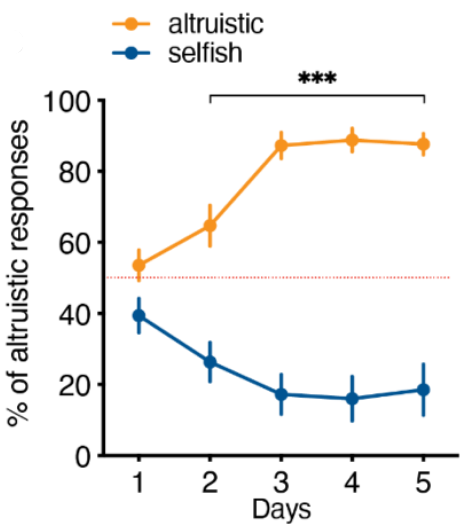
\includegraphics[width=\linewidth]{altr_self.png}
				
			\end{figure}
		\end{minipage}
		\hspace{0.05\linewidth}
		\begin{minipage}{0.46\linewidth}
			\begin{figure}[H]
				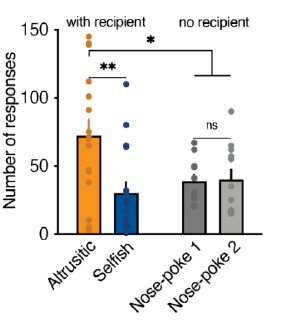
\includegraphics[width=\linewidth]{norecip.png}
				
			\end{figure}
		\end{minipage}
		
	\end{minipage}
	\caption{\textit{Left: Percentage of change in altruistic response (i.e in the number of altruistic pokes) for altruistic and selfish mice. Right: difference in number of altruistic and selfish pokes by the dictator when the recipient is present or not}}
\end{figure}



The first evident result of the altruism task is that, when a recipient mouse was present and same sex pairs adopted, the dictator mice showed an increase in the number of altruistic pokes during the test days. In contrast, when recipient mice were replaced by inanimate objects, no appreciable difference between altruistic and selfish preferences have been detected. Such differences started to emerge from the second day of the test, as confirmation of a successful learning period on the first day. \\
An important difference has been observed between male and female mice:  only male dictators showed altruism preference, while female ones did not show an appreciable difference between selfish and altruistic pokes.\\
Next, the spatial exploration of the mice has been performed. Results indicate that altruistic dictators (i.e.dictators which showed preference for altruistic pokes) tend to explore more the area in proximity to the recipient, in contrast with selfish dictators which did not show particular interest in their partners.\\
To test whether visual interaction plays a role determining the altruistic preferences, the task has been repeated replacing the metal mesh with an opaque screen, which still allowed olfactory and auditory stimuli, but not visual ones. In this situation, mice showed a marked decrease in the altruistic responses, with respect to the previous case in which a metal mesh was used. This implies that the dictator mouse needs to be able to see the recipient partner getting the food delivery, in order to be able to select the altruistic alternative.\\
Finally, to further determine the ability of the dictator mice to \textit{learn} from experience and change their habits in light of an altruistic choice, dictators were tested with no partner in adjacent cages, to trigger one nose poke over the other. Subsequently, the recipient mouse was put in the near cage, and the location of the altruistic poke, delivering food to it as well, has been assigned to the poke less pressed by the dictator. Despite this, the dictator showed through days a change in its preference towards the altruistic poke. Changing the recipient with an inanimate object, such preference decreased once again. The conclusion is straightforward: the presence of the recipient is the determining factor for the altruistic preference by the dictator.
\\

Once, in normal conditions, the altruistic preference has been established, one may ask under which conditions such preference is maintained. To this purpose, the task was repeated changing the rules of food delivering. Now, two nose pokes were necessary for the food delivery in the altruistic poke, while only one in the selfish one. Even with this additional effort, male and female mice which previously showed altruistic preferences, increased the number of altruistic over selfish preferences also in this case. Increasing the necessary number of pokes to $4$, male dictators kept their altruistic preferences, while female dictators did not show anymore a significant difference. Finally, requiring $6$ nose-pokes for altruistic delivery still kept male mice in their altruistic preference, while made female ones prefer the selfish one, and only from $8$ pokes, also males stopped to be altruistic. Overall, these results showed that \textit{male mice tend to share food with their cagemates partners, even at costly conditions}.\\
Finally, mice were tested in two more conditions: absence of rewards for both dictator and absence of reward for dictator, but not for the recipient mouse. While, in the first case, no preference between the two pokes was expressed by the dictator, in the second case there was an altruistic preference. This means that the dictator can choose an altruistic decision even if there is no direct benefit for itself.


\begin{figure}[H]
	\begin{center}
		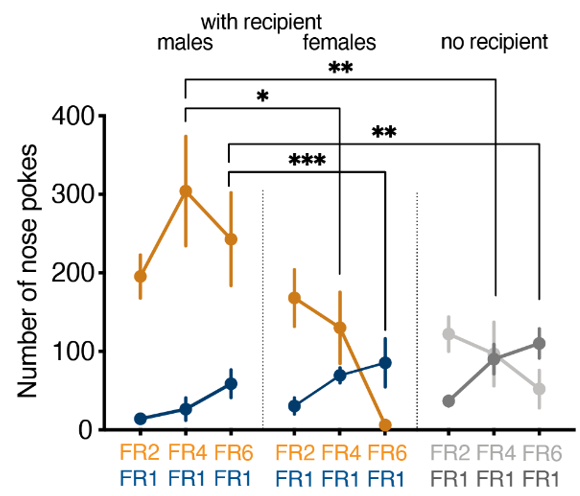
\includegraphics[scale=0.6]{number_pokes.png} 
	\end{center} 
	\caption{\textit{Number of nose pokes of male and female mice, with and without recipients.}}
	
\end{figure}

\subsection{The role of social hierarchy in altruism display}

\begin{figure}[H]
	\begin{center}
		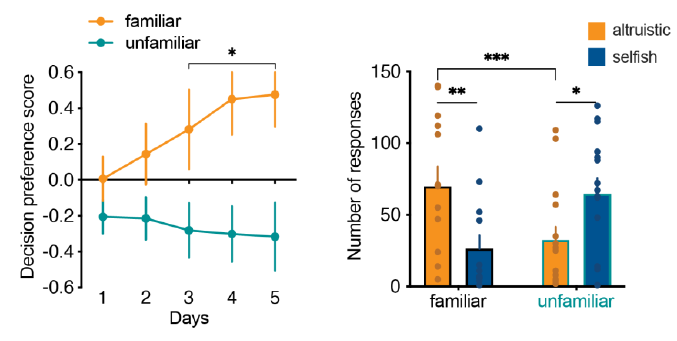
\includegraphics[scale=0.6]{familiar.png} 
	\end{center} 
	\caption{\textit{Left: decision preference score with familiar and unfamiliar recipients. Right: Number of responses by selfish and altruistic dictators, with familiar and unfamiliar recipients}}
	
\end{figure}

As of today, it has been recognized that familiarity between individuals plays a key role in social relationships [De Waal, F. B. M. \& Preston]. In the case of the altruism task, it is to be expected that the altruism shown by the dictator is strictly depending on the period preceding the test, in which dictator and recipient have been cagemates for two weeks. To test this hypothesis, the task has been repeated using unfamiliar recipients, showing no preference for altruistic choices, where indeed most of dictator mice showed preference for the seflish pokes. This has been measured through the \textbf{decision preference score} 

\begin{equation}
DPS = \frac{A -S}{A+S}
\end{equation}

where $A$ and $S$ are the number of altruistic and selfish responses, respectively.\\
Next, a \textit{dominant/follower} relationship has been established through the \textbf{tube test}, in which two mice have been paired in a tube allowing the passage of just one individual. This test helped to figure out whice of the two was the \textit{dominant} individual, i.e. the one pushing the other, and the \textit{follower} individual, i.e. the one retreating. The dominance was quantified through the \textbf{Normalized David's score} [De Vries, H., Stevens, J. M. G. \& Vervaecke]

\begin{equation}
NDS = \frac{1}{N}\left(DS + \frac{N(N-1)}{2}\right)
\end{equation}

where $N$ is the number of tested subjects and $DS$ is the David's score, i.e. the ratio of wins.\\
The analysis of 9 pairs of mice ($N=18$) yielded the main following results:

\begin{enumerate}
	\item The dominance relationship is \textit{transitive}: if mouse A is dominant with respect to mouse B, and mouse B is dominant with respect to mouse C, then mouse A dominates also mouse C 
	
	\item Dictator mice showing selfish preferences in the altruism task displayed low scores in the $NDS$ compared to their recipients, which means that selfish dictators  tend to be less dominant than their corresponding recipients
	
	\item No significant differences have been detected between the dominance scores of altruistic dictators and their recipients
	
	\item The more a dictator has a higher dominance value $NDS$, the more it is willing to perform altruistic preferences in the altruism task
	
\end{enumerate}

Next, the study tested the hypothesis that \textit{an increase in altruism is related to an increase in affective state matching between individuals}. To do so, the recipient has been subject to a manipulation of its emotional state, in this case a fear conditioning paradigm through mild shocks. In the meantime, the dictator mouse (here assuming the role of \textit{observer}) was allowed to see the recipient through a transparent separating wall.\\
The main result was that altruistic mice displayed an increased freezing behaviour during this phase, compared to selfish ones. Since these latter are the dominant ones, this result lead to the conclusion that \textit{dominant mice tend to show more empathic-like behaviours}, from altruism to emotional contagion.

\subsection{The role of BLA neurons in selfish and prosocial choices}

\begin{figure}[H]
	\begin{center}
		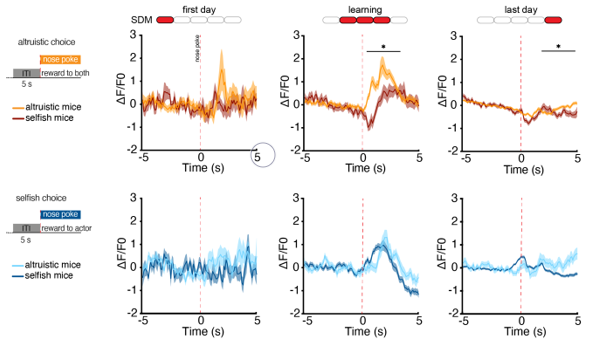
\includegraphics[scale=0.77]{psth.png} 
	\end{center} 
	\caption{\textit{Top row: PSTH of selfish and altruistic mice during nose pokes in altruistic pokes. Bottom row:  PSTH of selfish and altruistic mice during nose pokes in selfish pokes. Results have been averaged on all nose pokes}}
	
\end{figure}

The fiberphotometry analysis of the calcium activity in the BLA allowed to establish a connection between the type of choice adopted by dictator mice and their corresponding neural activity. In order to analyze the relative change of such activities during altruistic or selfish pokes, the raw data from the photometry have been subject to a \textbf{peristimulus time histogram (PSTH)} analysis. Such analysis goes through the following steps:

\begin{enumerate}
	
	\item Set a START and STOP time for the analysis, i.e. set the time window in which considering the variation of the neural activity (in this case START = STOP = $5 s$ for a window of $10 s$)
	
	\item For every time point $x_t$ of the overall activity given by Fiberphotometry, consider the interval $[x_{t}-START , x_{t}+STOP]$
	
	\item Compute the mean $ \mu_t$ and standard deviation $\sigma_t$ of the activity in such interval
	
	\item The value of the PSTH for the selected time point is then
	$$ P_t = \frac{x_t - \mu_t}{\sigma_t}$$
\end{enumerate}
Next, in order to quantify the intensity of the activity, \textbf{areas under the curve (AUC)} were estimated numerically using the trapezoid quadrature rule [Quarteroni-Sacco].\\

The overall analysis on raw photometry data, PSTH tracks and AUC showed some remarkable results:

\begin{itemize}
	
	\item Dictator mice showed an increased activity in the BLA when a recipient mouse was present, compared to the case where an inanimate object was placed in the near cage
	
	\item During the first and last day, in all cases no significant differences emerged in the activation of BLA
	
	\item In the intermediate days of learning, however, altruistic mice showed a strong activation during the nose poking in the altruistic pokes, but not in the selfish ones. Selfish mice, in contrast, did not show any particular activation of their neural activity during both pokes. 
	
	\item The AUC analysis suggested that the levels of activity were higher during the learning phase, rather than in the first and last day
\end{itemize}


To further inspect the role of BLA neurons in empathy display, such neurons have been silenced via a \textbf{chemogenetic procedure} [Qi-Gang Zhou, Ashley D Nemes]. In this approach, a viral vector, carrying specific receptors, is injected into the area of interest. Such receptors, called  \textbf{hM4D receptors}, belong to the group of \textit{inhibitory designer receptors exclusively activated by designer drugs (DREADD)}, which activate themselves only when in contact with a particular drug, the \textbf{Clozapine N-oxide (CNO)}. In this way, mice injected with hM4D-CNO will exhibit an \textit{inhibition} of BLA-neurons. In contrast a control group of mice was injected with CNO only, without hM4D receptors.\\
The obtained results after these injections showed a significant reduction of freezing behaviour in the dictators, while their recipient partners were subject to emotion conditioning as previously described. This confirms the conclusions of previous studies [Allsop, S. A. et al], namely a \textit{critical role of the amygdala in emotional matching}. Silencing BLA neurons revealed to be correlated also to the amount of altruism preferences. Indeed, mice with silenced BLA neurons failed to show a marked preference for altruistic choices, in contrast with the control case. Indeed, while approximately $3$ out of $4$ mice showed altruistic preferences in control conditions, a similar percentage of BLA-silenced mice showed preference for selfish pokes.\\
BLA silencing did not affect the number of responses or the latency of choices, rather it affected the type of the social decision. This is a further evidence of the primary role of BLA in altruism display.
\\
Finally,  silencing of BLA neurons appeared to reduce also the dominance: a higher number of BLA-silenced mice assumed a subordinate role with respect to control mice. In particular, if transitive relationships of dominance are distributed in levels $ \alpha \rightarrow \beta \rightarrow \gamma \rightarrow \delta $, silenced mice belong only to levels $ \gamma $ and $ \delta $.

\begin{figure}[H]
	\begin{center}
		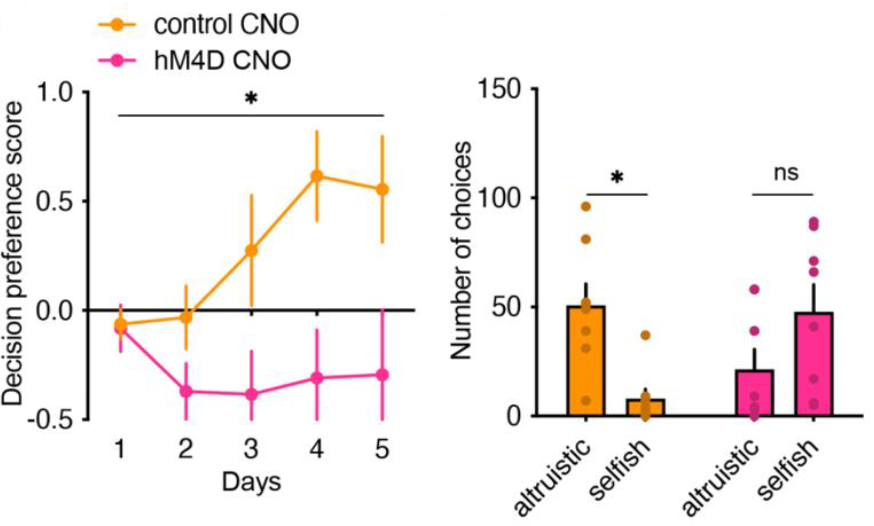
\includegraphics[scale=0.77]{silencing.png} 
	\end{center} 
	\caption{\textit{Left: Decision preference score in BLA-silenced mice (hM4D CNO) and non-silenced mice (control CNO). Right: number of selfish and altruistic pokes in BLA-silenced mice (hM4D CNO) and non-silenced mice (control CNO) }}
	
\end{figure}


\begin{figure}[H]
	\begin{center}
		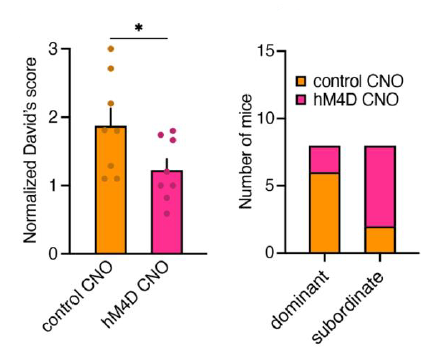
\includegraphics[scale=0.77]{sil_dom.png} 
	\end{center} 
	\caption{\textit{Left: Normalized David's score in BLA-silenced mice (hM4D CNO) and non-silenced mice (control CNO). Right: number of dominant and subordinate mice in BLA-silenced mice (hM4D CNO) and non-silenced mice (control CNO) }}
	
\end{figure}

\section{Mathematical modeling for electrophysiology}

In Section 1.1, the concept of \textit{excitability} of neurons has been introduced: neurons are able to generate and transmit \textbf{electrical impulses} as reaction to external stimuli. These impulses are a direct consequence of rapid changes in intracellular end extracellular \textit{ionic concentrations} of main elements such as $Na^+, Cl^-, K^+, Ca^{2+}$. The change in such concentrations determines a change in the potential crossed across the cell's membrane, and the formation of an \textbf{action potential}. \\
In this chapter, mathematical models to describe the behaviour of such quantities are presented. After having introduced the main assumptions of the model, the equivalent circuit formulation for cellular electryphyioslogy will be presented, along with different models to describe its electrical components. Finally, the main model to describe the propagation of the action potential between different neurons will be under study, namely the \textbf{cable equation model}. These models consist \textbf{ordinary differential equations (ODEs)} or \textbf{partial differential equations (PDEs)}, to be numerically solved through appropriate technqiues.

\subsection{Electrical activity in neurons}

\begin{figure}[H]
	\begin{center}
		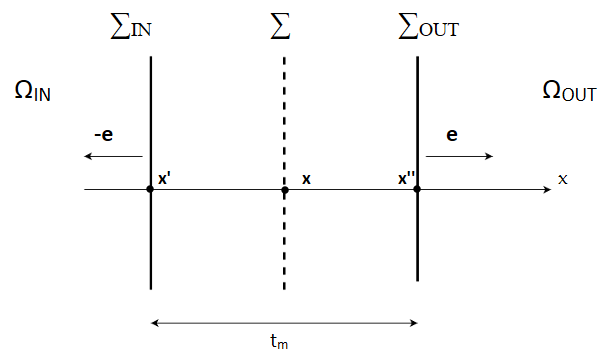
\includegraphics[scale=0.77]{intra.png} 
	\end{center} 
	\caption{\textit{Schematic model of a cellular membrane}}
	
\end{figure}

From a biological point of view, the different ionic concentrations, assumed inside and outisde the neuron, give rise to a \textit{passive transport} of ions, which moves accordingly to the \textit{electrochemical gradient} (i.e. movement of positive charges from high to low potentials). The passage of ion species across the membrane can be allowed or denied by \textbf{ionic channels}, each of one designed  for a specific ion. The passive trasnport is not the only mechanism of ionic transport. Indeed, thanks to special \textbf{ionic pumps}, the cell is able to perform an \textit{active} transport, moving ions against the electrochemical gradient. In order to do this, the cell needs to consume energy, in form of \textit{ATP}.\\
Let us consider a geometrical setting representing the relevant components of a neuron for its electrical activity: an intracellular region $ \Omega_{in}$ and an extracellular region $\Omega_{out}$. The two regions are separated by the cell's membrane, presenting internal and external surfaces $\Sigma_{in}$ and $\Sigma_{out}$. Finally, define the normal versors to  $\Sigma_{in}$ and $\Sigma_{out}$ as  $\textbf{n}_{in}$  and  $\textbf{n}_{out} = - \textbf{n}_{in}$.\\

Under this setting, we define the \textbf{total ionic current density} of ion $\alpha$ as

\begin{equation}
J_{\alpha,i}^{TOT} =	\textbf{J}_{\alpha,i}^{TOT} \cdot \textbf{n}_{i} = J^{cond}_{\alpha,i} + J^{cap}_{\alpha,i} \hspace{2cm} i= in,out
\end{equation}


The total current density is formed by two contributions:

\begin{itemize}
	
	\item \textbf{Conduction current} $J^{cond}_{\alpha}$: the current formed by the conudction of ions along the ionic channels. We assume no loss of current inside the channel, so that $J^{cond}_{\alpha, in} = J^{cond}_{\alpha, out}$
	
	\item \textbf{Capacitive current} $J^{cap}_{\alpha}$: the current formed by the charge accumulation in $\Sigma_{in}$ and $\Sigma_{out}$. The charge accumulation makes the membrane behave like a \textit{capacitor}. Thus, we assume 
	\begin{equation}
	J^{cap}_{\alpha,i} = \frac{\partial \sigma_{\alpha,i}}{\partial t}  \hspace{2cm} i= in,out
	\end{equation}
	
	where $\sigma_{\alpha,i}$ is the \textbf{surface charge density}. Also in this case we require \textit{wall's neutrality}
	
	\begin{equation}
	\sigma_{\alpha,in} = \sigma_{\alpha,out}
	\end{equation}
\end{itemize}	

The neutrality conditions on conduction and capacitive current implies current conservation 

\begin{equation}
J_{\alpha,in}^{TOT} = J_{\alpha,out}^{TOT}
\end{equation}

Considering two points $ \textbf{x}' \in \Omega_{in}$ and $ \textbf{x}'' \in \Omega_{out}$ and a time interval $ [0,T]$, we can consider the electric potentials $ \psi^{in} (t) = \psi(\textbf{x}',t) $ and  $ \psi^{out} (t) = \psi(\textbf{x}'',t) $, assuming the potentials constant respectively in $\Omega_{in}$ and $\Omega_{out}$. The \textbf{membrane potential} is then defined as

\begin{equation}
\psi_m (t) = \psi^{in} (t) -  \psi^{out} (t) \hspace{1 cm}  t \in [0,T]
\end{equation}


The existence of the membrane potential is consequence of the Faraday's equation (known as well as Maxwell's third equation)

\begin{equation}
\nabla \wedge \textbf{E} = -\frac{\partial \textbf{B}}{\partial t}
\end{equation}

where $\textbf{E}$ and $\textbf{B}$ are the elctric and magnetic field, respectively. In the microscopic cellular environment, it happens in practice that $ \left| \frac{\partial \textbf{B}}{\partial t} \right| << \left| \nabla \wedge \textbf{E}\right|$, being the magnetic contribution negligible qith respect tot he electric one. This implies from (2) that $\nabla \wedge \textbf{E} = 0 \implies \exists \psi s.t. \textbf{E} = -\nabla \psi$.\\
If $R_c$ and $t_m$ are, respectively, the cell's radius and the membrane's thickness, in practice we have that their ratio $ \eta_c := \frac{t_m}{R_c} << 1$. This implies that from a modeling point of view we can assume $t_m \sim 0 $, i.e. we can neglect the thickness of the membrane and assume $\Sigma_{in} \sim \Sigma_{out} \sim \Sigma$. In practice, for example, realistic values of such quantities can be $ R_c \sim 10^{-6} m$, $ t_m \sim 10^{-9} m$ and thus $\eta_c \sim 10^{-3}$.\\
If $\epsilon_m$ is the membrane's \textit{dielectric constant}, we can define the \textbf{specific capacitance} of the membrane as $ c_m = \frac{\epsilon_m}{t_m}$. Assuming then that the surface charge densities have the form $\sigma_{in}(\textbf{x}',t) = c_m \psi_m (\textbf{x},t)) $ and  $\sigma_{out}(\textbf{x}'',t) = -c_m \psi_m (\textbf{x},t) $, where $\textbf{x} \in \Sigma$. The capacitive current density (2) assumes the form

\begin{equation}
J^{cap}_{\alpha,i}(\textbf{x},t) = c_m \frac{\partial \psi_m(\textbf{x},t)}{\partial t}  \hspace{1cm} t \in [0,T], \textbf{x} \in \Sigma
\end{equation}


\subsection{ODE local and global models}

\begin{figure}[H]
	\begin{minipage}{\linewidth}
		\centering
		\begin{minipage}{0.45\linewidth}
			\begin{figure}[H]
				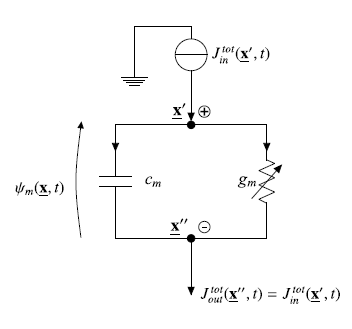
\includegraphics[width=\linewidth]{ode_circuit.png}
				
			\end{figure}
		\end{minipage}
		\hspace{0.05\linewidth}
		\begin{minipage}{0.48\linewidth}
			\begin{figure}[H]
				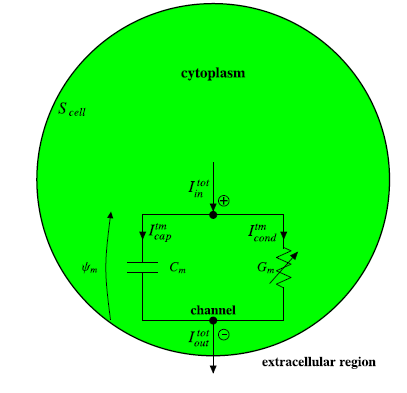
\includegraphics[width=\linewidth]{global_circuit.png}
				
			\end{figure}
		\end{minipage}
		
	\end{minipage}
	\caption{\textit{Left: equivalent circuit for a fixed point $\textbf{x} \in \Sigma$ (local model)  \\
			Right: equivalent circuit for the all membrane  $\Sigma$ (global model)}}
\end{figure}


Let us now consider a specific $\textbf{x} \in \Sigma$. Then, equation (1) expresses a balance law for the current densities $J_{\alpha,i}^{TOT}, i= in,out$, which can be divided in two contributed (capactive and conductive), where the capacitive current assumes the form $J^{cap}_{\alpha,i}(t) = c_m \frac{\partial \psi_m(t)}{\partial t}$.\\
As for the conductive current, we consider a general form 

\begin{equation}
J^{cond}_{\alpha,i} = g_m(\textbf{x},t,\psi_m) [\psi_m - E_{eq}]
\end{equation}

where $g_m$ plays the role of a \textbf{specific conductance}, a priori nonlinear in $\psi_m$, and $E_{eq}$ is the equilibrium ptoential assumed across the cell, both to be modeled.\\
Therefore, equation (1), expressed for the unknwonn $\psi_m$, can be seen  in an equivalent \textit{circuital form}, in which the two contribution of the current densities are model respectively through a specific capacitance and a specific conductance. Then, the conservation of current will be a consequence of Kirchhooff laws (Figure 2).
\\


If instead of a specific $\textbf{x} \in \Sigma$, the aim is to write equation (1) as a current balance in all the cell's membrane $\Sigma$, the resulting differential equation, which in this case is a \textit{global} whole cell model, is obtained by integration of (1) over the surface $\Sigma$, in which the conservation becomes for a current $$ I_{\alpha}^{TOT} = \int_{\Sigma} \textbf{J}_{\alpha}^{TOT} \cdot \textbf{n}_{out} dS $$
The spoecific conductance and capacitance will become global conductance and  capacitance $ G_m [\Omega^{-1}]$ and $ C_m [F] $. Finally, the current balance takes the form

\begin{equation}
I_{\alpha}^{TOT} = I_{\alpha,in}^{TOT} =I_{\alpha,out}^{TOT} = I_{\alpha}^{cap} + I_{\alpha}^{cond}
\end{equation}

where $  I_{\alpha}^{cap} = C_m \frac{\partial \psi_m(\textbf{x},t)}{\partial t}$ and $ I_{\alpha}^{cond} = G_m(\textbf{x},t,\psi_m) [\psi_m - E_{eq}]$.\\
While the (specific) capacitance is an itnrinsic value of the cell, the conduction current, and  in particular the (specific) conductance $G_m$ needs to be modeled. In the next sections, three main model used in literature will be presented: the \textbf{linear resistor model (LRM)}, the \textbf{Goldman-Hodgkin-Katz (GHK)} model and finally the \textbf{Hodgkin-Huxley (HH)} model.



\subsection{LRM and GHK models}

\begin{figure}[H]
	\begin{center}
		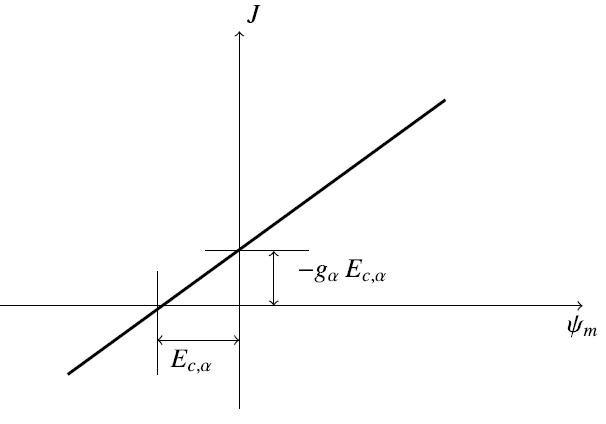
\includegraphics[scale=0.77]{LRM.png} 
	\end{center} 
	\caption{\textit{Characteristic curve in the $(\psi_m,J)$ plane for the linear resistor model}}
	
\end{figure}

The \textbf{linear resistor model (LRM)} makes the simplest assumptions of

\begin{equation}
G_{m,\alpha} = G_{m,\alpha}^0 = const \hspace{1.5 cm} E_{eq} := E_{m,\alpha}^0 = const \hspace{1cm} \forall \alpha
\end{equation}

Therefore, the conductance is assumed constant, as well as the equilibrium value of the potential $E_m^0 $, called the \textbf{Nernst potential}.
The resulting expression for the conduction current is
\begin{equation}
I_G(t) = G_{m,\alpha}^0 [\psi_m -  E_{m,\alpha}^0]
\end{equation}

This law defines a straight line in the plane $I_G$ vs $\psi_m$, such that there exists a unique value of potential in which $I_G=0$. This value is exactly the Nernst potential $E_m^0$ and thus it represents a \textit{thermodynamic equilibrium} in which the ion flow from outisde to inside of the cell is balanced with the ion flow from inside to outside and the net current is null.\\
Considering local ODE models, the procedure is the same applied to the specific electrical quantities:

\begin{equation}
g_{m,\alpha} = g_{m,\alpha}^0 = const \hspace{1.5 cm} E_{eq} := E_{m,\alpha}^0 =const 
\end{equation}

resulting in a current density
\begin{equation}
J_G(t) = g_{m,\alpha}^0 [\psi_m -  E_{m,\alpha}^0]
\end{equation}


In order to determine an expression for the Nernst potential $E_{m,\alpha}^0$, in which thermodynamic equilibrium is achieved, we should investigate the causes of equiloibrium at a deeper level, namely in the process of ion flow in the channels of the membrane. From standard theory [REF?] it is known that ion particles in the channel are subjected to two different contributions: diffusion process caused by the electrochemical gradient, and a transport caused by the presence of an \textit{electrical field} $\textbf{E}(\textbf{x},t)$. This originates the well known \textbf{drift-diffusion (DD)} model for the ionic current density [REF?], which reads

\begin{equation}
\textbf{J}_{\alpha}^{TOT} = \textbf{J}_{\alpha}^{DIFF} + \textbf{J}_{\alpha}^{DRIFT} = -Fz_{\alpha}D_{\alpha}\nabla C_{\alpha} + F|z_{\alpha}| C_{\alpha}\mu_{\alpha}\textbf{E}
\end{equation}
where the following quantities have been defined:
\begin{itemize}
	
	\item $F$: the \textbf{Faraday constant}, such that $F = q N_{av}$
	
	\item $z_{\alpha}$ is the \textbf{ion number}
	
	\item $\mu_{\alpha}$ is the \textbf{ion electrical mobility}
	
	\item $C_{\alpha}$ is the concentration of ion $\alpha$
	
	\item $D_{\alpha}$ is the \textbf{ion diffusivity}. this value can be retrieved from the \textit{Einstein-Smoluchowki} relation [REF?] $D_{\alpha} = V_{TH}\frac{\mu_{\alpha}}{|z_{\alpha}|}$, where $ V_{TH} \sim 26 mV$ is the \textit{thermal voltage}
\end{itemize}

Assuming one dimensionality, being that $ E -\frac{\partial \psi}{\partial x}$ and using the Einstein-Smoluchowki relationship, we can prove that the thermodynamic equilibrium, for which $\textbf{J}_{\alpha}^{TOT} = 0$ and thus the drift component balances the diffusion one, is obtained at the value of potential

\begin{equation}
E_{m,\alpha}^0 = \frac{V_{TH}}{z_{\alpha}}\ln\left(\frac{C_{\alpha}^{OUT}}{C_{\alpha}^{IN}}\right)
\end{equation}

which provides the seeked expression for the Nernst potential.
\\

With the \textbf{Goldman-Hodgkin-Katz (GHK)} model, the modeling of the conduction current becomes nonlinear. Here, the following assumptions are adopted: 

\begin{itemize}
	
	\item The electric field in the ionic channels assumes a constant value of $ E = \frac{\psi_m}{t_m}$, i.e. the ratio between the membrane potential and the membrane's thickness
	
	\item The geometrical setting is one dimensional
	
	\item The conduction current $\textbf{J}_{\alpha}^{cond}$ varies only in time, i.e. is constant in space and $ \frac{\partial J_{\alpha}^{cond} }{\partial x} = 0$. This means that there is no production or consumtpions of ions along the channel
	
\end{itemize}

Applying these hypothesis to the current density in (DD) form 
$$ J_{\alpha}^{cond} =  -Fz_{\alpha}D_{\alpha}\nabla C_{\alpha} + F|z_{\alpha}| C_{\alpha}\mu_{\alpha}\textbf{E} $$
it can be seen that the in order to have $ \frac{\partial J_{\alpha}^{cond} }{\partial x} = 0$, the current density must assume the form

\begin{equation}
J_{\alpha}^{GHK}(\psi_m,t) = -qz_{\alpha}P_{\alpha}\left[n_{\alpha}^{out} \mathcal{B}(\beta_m) - n_{\alpha}^{in} \mathcal{B}(-\beta_m) \right]
\end{equation}

where $P_{\alpha} = \frac{D_{\alpha}}{t_m}$ is the \textbf{membrane's permeability}, $ \beta_m := \frac{z_{\alpha} \psi_m}{V_th}$ and $ \mathcal{B}(x) = \frac{x}{e^x -1}$ is the \textbf{Bernouilli function}.\\
It can be proven [Sacco-Guidoboni] that this expression can be written in a nonlinear resistor form in which

\begin{equation}
g_{\alpha}(\psi_m,t) = P_{\alpha}\frac{q z_{\alpha}^2N_{av}C_{\alpha}^{in}}{V_{TH}} 
\end{equation}

\begin{equation}
E_eq(\psi_m,t) = P_{\alpha}\frac{V_{TH}}{z_{\alpha}} \left(\frac{C_{\alpha}^{out}}{C_{\alpha}^{in}} - 1\right)\mathcal{B}(\beta_m)
\end{equation}



\subsection{Hodgkin-Huxley model}

\begin{figure}[H]
	\begin{center}
		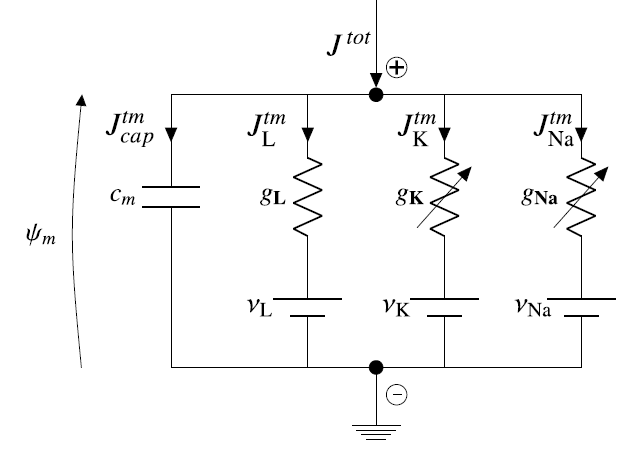
\includegraphics[scale=0.9]{HH.png} 
	\end{center} 
	\caption{\textit{Equivalent circuit for the Hodgkin-Huxley model}}
	
\end{figure}


In 1963, Hodgkin and Huxley pusblished in a paper a revolutionary work, which will be worth the Nobel prize, on mathematical modeling for the electrophyisiogical activity, with the focus on the neurons of the giant squid [Hodgkin-Huxley]. The main structure of the model follows the principle discussed so far, in which an equivalent circuit represents the ion flow between the cell's membrane. The main assumptionns and particularities of the model can be resumed as follows:

\begin{itemize}
	
	\item The total current density $J^{tot}$ can be split in two contributions: a capacitive transmembrane current $J_{cap}^{tm} = c_m \frac{\partial \psi_m}{\partial t}$, where the capacitance is assumed linear, and, for every ion considered, a conduction current to be modeled. The main ions considered are \textit{potassium} ($K^+$) and \textit{siodium} ($Na^+$). The remainant contribution is mostly due to \textit{chlorine} ($Cl^-$) and it is summarized in a \textit{leakage} current $J_L^{tm}$
	
	\item For every ion $\alpha$ is associated its Nernst potential $E_{m,\alpha}$, representing the value on which thermodynamic equilibrium is achieved and the flow from inside to outisde the cell is balanced with the flow from outside to inside
	
	\item A new level of complexity is considered: in order to better describe what happens at a biological level, the ionic channel have a \textit{state}, i.e. an associated probability value which tells the percentage of their opening. Indeed, the behaviour of ionic exchange between the cytoplasm and the exterior of a cell, strongly depends on the closing and opening of the ionic channel. With the HH model, the attempt is to mathematrically describe the status of the channel along time
	
	
\end{itemize}	


In the original form of the paper, a change of variable is performed: let's define the equilibrium potential of the whole cell as $E_m$, and define for every ion $\alpha$ the quantities

\begin{equation}
v_\alpha := E_{m,\alpha} - E_m \hspace{2cm}  v := \psi_m - E_m
\end{equation}

In this way, the form of the current density of ion $\alpha$ becomes


\begin{equation}
J_\alpha^{cond} = g_{m,\alpha}(v-v_\alpha)
\end{equation}

and the current conservation equation, expressed for the new variable $v = v(t)$, is

\begin{equation}	
\begin{cases}
J^{tot} = J_{cap}^{tm} + J_{cond}^{tm} = c_m \frac{\partial v}{\partial t} + g_{Na}(v - v_{Na}) + g_{K}(v - v_{K}) +g_{L}(v - v_{L})  \\
v(0) = 0
\end{cases}	\end{equation}


Having assumed the membrane potential at equilibrium at time $t=0$.\\
For the whole ewuilibrium potential $E_m$, the choice can be on the \textbf{Goldman potential}[REF?]


\begin{equation}
E_m= V_{TH} \ln \left[\frac{P_{Na} C_{Na}^{out} + P_{K} C_K^{out} + P_{Cl} C_{Cl}^{in}}{P_{Na} C_{Na}^{in} + P_{K} C_K^{in} + P_{Cl} C_{Cl}^{out}}\right]
\end{equation}

where $P_\alpha$ and $C_\alpha$ stand respecitevly for the permeability and concentration of ion $\alpha$.\\
As for the modeling of conductances, let's introduce the \textbf{gating variables} $n,m,h$ for the three types of ions considered $K^+,Na^-,Cl^-$. They represent the probability of opening of the ionic channel. For example, if the cell is in a situation for which $C_{Na}^{out} > C_{Na}^{in}$, the opening of $Na^+$ channel will result in a current flow from outside to inside, and corresponing rise of the potential $\psi_m$. When the membrane potential reaches the value of equilibrium $E_{Na}$, the sodium channel will close. For this reason, the gating variables are expressed as solution of ordinary differential equation of the type

\begin{equation}
\frac{dy}{dt} = \gamma (1-y) - \delta y \hspace{1 cm} \gamma,\delta >0  \hspace{1 cm} y = m,n,h
\end{equation}

so that there is a balance between a production rate $\gamma$ and a consumption $\delta$. The solution of an ODE in this form is

\begin{equation}
y(t) = y_\infty \left[1 - \exp\left(\frac{-t}{\tau}\right)\right]
\end{equation}

where

\begin{equation}
y_\infty = \frac{\gamma}{\gamma + \delta} \hspace{1.5cm} \tau = \frac{1}{\gamma + \delta}
\end{equation}

For the potassium conductance, the chosen dependence on its gating variable (in agreement qith experimental data) is $ g_K = \bar{g}_K n^4$. For the sodium variable, it has been observed that also a second process was involved, so that the proposed form is  $ g_{Na} = \bar{g}_{Na} m^3h$. The values $\bar{g}_K$ and $\bar{g}_K{Na}$ are constant and derived experimentally (è vera sta cosa?).\\
To summarize the HH model consists in the following sytem of nonlinear ordinary differential equations:

\begin{equation}
\begin{cases}
J^{tot} = c_m \frac{d v}{d t} + J_{Na} + J_K +J_L  & \text{(Current conservation)}\\
J_\alpha = g_\alpha (v-v_\alpha) \hspace{1 cm}  \alpha = Na,K,Cl & \text{(Modeling currents)}\\
\frac{dn}{dt} = \gamma_n(1-n) - \delta_n n & \text{(ODE for gating variable n)} \\
\frac{dm}{dt} = \gamma_m(1-m) - \delta_m m & \text{(ODE for gating variable m)}\\
\frac{dh}{dt} = \gamma_h(1-h) - \delta_h h & \text{(ODE for gating variable h)}\\
g_K = \bar{g}_K n^4 & \text{(Modeling conductance for K)}\\
g_{Na} = \bar{g}_{Na} m^3h  & \text{(Modeling conductance for Na)}

\end{cases}
\end{equation}

\begin{figure}[H]
	\begin{center}
		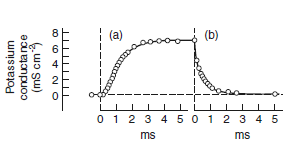
\includegraphics[scale=1.1]{gk.png} 
	\end{center} 
	\caption{\textit{Example of behaviour of the potassium conductance $g_k$: a step increase is followed by a decrease. The dots are experimental data}}
	
\end{figure}


\subsection{Cable model}

\begin{figure}[H]
	\begin{center}
		\hspace*{-0.7cm}
		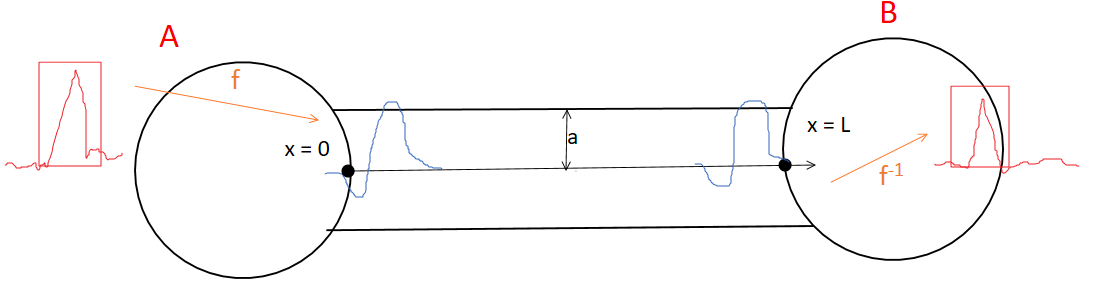
\includegraphics[scale=0.7]{cable.png} 
	\end{center} 
	\caption{\textit{Schematic representation of the cable model}}
	
\end{figure}


The models studied so far described the evolution of the membrane potential along time for a single cell. In order to go further, we should keep into account as well the \textit{communication} between two cells, i.e. the propagation of the action potential from one neuron to another. Biologically, this is done through the \textit{axon} connecting the two units. The axon is still parti of the neuron, and in every point we may assume a communication with the oustide environment thorugh electrical circuits as decribed in previous sections.\\
The main assumptions for the cable model are the followings:

\begin{itemize}
	
	\item The bilogical cable, i.e. the axon, has length $L$ and radius $a$ (thus basis surface $S=\pi a^2$), with $\frac{a}{L} << 1$, allowing to represent the cable as a $1D$ object and fix an ascissa $ x \in [0,L]$
	
	\item We will assume the potential outside the cell as constant, as well as the concentrations inside and outside the cell for every ion $\alpha$: 
	$$ \psi^{out}(x,t) = const  \hspace{1cm} C_\alpha^{in}(x,t)  = const \hspace{1cm} C_\alpha^{out}(x,t)  = const$$
	
	\item The \textbf{resistivity} of the axon $\rho_{ax}$ is constant. The resitivity is the reciprocal of the \textit{conducitivity} $\sigma$, and its relkated to the \textit{resistance} $R_{ax}$ by $ R_{ax} = \frac{\rho_{ax} L}{S}$
	
	
\end{itemize}


If we consider an element of length $dx$ of the cable, its contribution to resistance is $dR(x) = \frac{\rho_{ax} dx}{\pi a^2}$. If a current $I_{in}$ enters the element, the consequent potential formed across the element is $ d\psi_m(x,t) = dR(x)I_{in}(x,t) = \frac{\rho_{ax} dx}{\pi a^2} I_{in}(x,t)$. Therefore, letting $dx \rightarrow 0$, this implies that

\begin{equation}
I_{in}(x,t) = -\frac{\pi a^2}{\rho_{ax}}\frac{\partial \psi_m(x,t)}{\partial x}
\end{equation}

Next, in order to retrieve a current balance along the axon, let's consider again an infinitesimal element $dx$, in which a current a current $I_{in}(x,t)$ is entering the element, a current $I_{in}(x+dx,t)$ is leaving the element, and finally a transmembrane current $I_{TM}(x+\frac{dx}{2},t)$ flowing from the axon to the outside cellular envornment, with a capacitive and a conduction contributions [ee Figure].\\
A Kirchhoff law applied to the node at $x+\frac{dx}{2}$ reads

\begin{equation}
- I_{in}(x,t) + I_{cap}(x+\frac{dx}{2},t) + I_{cond}(x+\frac{dx}{2},t) + I_{in}(x+dx,t) = 0
\end{equation}

The capactive and conductive contributions to the transmembrane current read
\begin{equation}
I_{cap}(x+\frac{dx}{2},t) = J_{cap}(x+\frac{dx}{2},t) 2 \pi a dx = c_m \frac{\partial \psi_m(x,t)}{\partial t} 2 \pi a dx 
\end{equation}

\begin{equation}
I_{cond}(x+\frac{dx}{2},t) = J_{cond}(x+\frac{dx}{2},t) 2 \pi a dx 
\end{equation}

With $J_{cond}$ to be modeled, for example with LR,GHK or HH. Dividing equation (28)  for $2 \pi a dx $ and letting $dx \rightarrow 0$ gives the equation

\begin{equation}
\begin{cases}
\frac{\partial \psi_m(x,t)}{\partial t} + \frac{1}{2 \pi a }\frac{\partial I_{in}(x,t)}{\partial x} + J_{cond}(x,t) = 0 \\
I_{in}(x,t) = -\frac{\pi a^2}{\rho_{ax}}\frac{\partial \psi_m(x,t)}{\partial x}
\end{cases}
\end{equation}

The resulting equation is a \textit{parabolic partial differential equation}, in which the unknown membrane potential $\psi_m(x,t) $ varies along the axon and along time, and it appears under first derivative in time and second in space. In order for (31) to be well-posed, the system has to be completed with an initial condition $ \psi_m (x,0) = \psi_m^0(x)$ and apprpriate boundary conditions. The nature of the cable equation will be linear or nonlinear depending on the chosen model for $J_{cond}$.\\
As for boundary conditions, a common choice is to consider \textit{Robin boundary conditions}. Defining the potential at $x=0$ as $\bar{V}_{in}(t)$ and model the terminal of the axon through a resistance $R_{out}$, the resulting boundary conditions are

\begin{equation}
\begin{cases}
\psi_m(0,t) = \bar{V}_{in}(t) \\
-I_{in}(L,t) +\frac{1}{R_{out}}\psi_m(L,t) =0
\end{cases}
\end{equation}

\begin{figure}[H]
	\begin{center}
		
		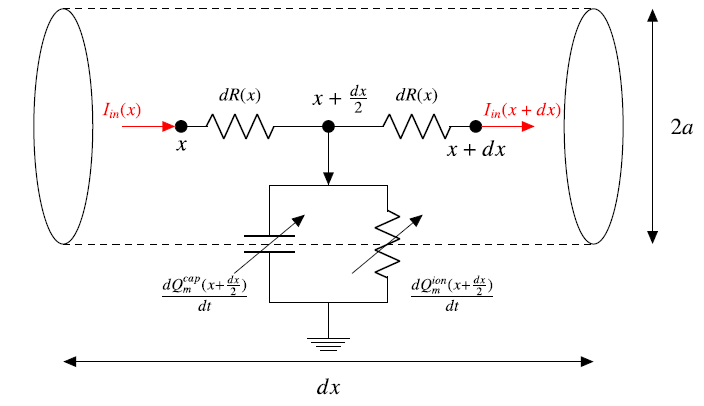
\includegraphics[scale=0.5]{curr_bal.png} 
	\end{center} 
	\caption{\textit{Current balance in an element $dx$ of the axon}}
	
\end{figure}

\subsection{Numerical solution of the cable equation}


\begin{figure}[H]
	\begin{center}
		
		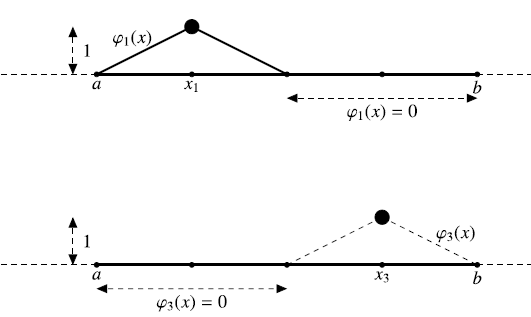
\includegraphics[scale=0.7]{basis.png} 
	\end{center} 
	\caption{\textit{Lagrangian basis functions}}
	
\end{figure}


The cable equation is a one dimensional \textit{advection-diffusion-reaction} PDE. A well posed problem of this type, for a general unknwons $ u(x,t)$ and $\textbf{J} = J(x,t)\textbf{e}$, can always be written under the following form of \textbf{conservation law}:


\begin{equation}
\begin{cases}
\frac{\partial u}{\partial t} +\frac{\partial J}{\partial x} = \mathcal{P} & \forall (x,t) \in [0,L] \times [0,T] \hspace{1cm} \text{(Conservation law)} \\
J = u v - \mu \frac{\partial u}{\partial x} & \forall (x,t) \in [0,L] \times [0,T] \hspace{1cm} \text{(Flux law)}\\
u(x,0) = u^0(x) & \forall x \in [0,L] \hspace{1cm}  \text{(Initial condition)} \\
\gamma \textbf{J} \cdot \textbf{n} = \alpha u - \beta &  \forall (x,t) \in \partial \Omega \times [0,T] \hspace{1cm} \text{(Boundary conditions)}
\end{cases}
\end{equation}

Here, $\textbf{J}$ J represents a \textit{flux} taking into account advection and diffusion, while $\mathcal{P}$ takes into account the reaction (i.e. net production rate). The boundary coefficients $\alpha, \beta, \gamma$, depending on their values, can give rise to the main types of boundary conditions (Dirichlet, Neumann, Robin).\\
In order to numerically solve equation (33), the following two main steps need to be performed:

\begin{enumerate}
	\item \textbf{Time semidiscretization}. The time derivative is apporximated with a finite-difference scheme. In the present case, the \textbf{Backward Euler method (BE)} is chosen, being unconditionally stable [Quarteroni-Sacco]. Dividng the interval $[0,T]$ in $N_T$ subintervals of the form $[t^k, t^{k+1}]$ with $ k=0, \dots N_T-1$, and setting $\Delta t = \frac{T}{N_T} $, the semidiscretization of (33) using BE reads
	
	\begin{equation}
	\begin{cases}
	\frac{u^{k+1} - u^k}{\Delta t} +\frac{\partial J^{k+1}}{\partial x} = \mathcal{P}^{k+1}  \\
	J^{k+1} = u^{k+1} v^{k+1} - \mu \frac{\partial u^{k+1}}{\partial x} 
	\end{cases}
	\end{equation}
	
	where, for a scalar quantity $\phi(x,t)$, it has been used the notation $ \phi(x,t^k) = \phi^k$. The first equation of (34) can be rewritten as
	
	\begin{equation}
	\sigma ^{k+1} u^{k+1} +\frac{\partial J^{k+1}}{\partial x} = f^{k+1} 
	\end{equation}
	
	\item \textbf{Spatial discretization}. A Galerkin-FEM strategy is adopted to solve the equation (34). From standard theory [Quarteroni], setting $V = H_0^1(\Omega)$, the variational problem can be rewritten in its \textit{variational form}
	
	\begin{equation}
	\text{Find $u \in V$ s.t.} \hspace{0.5cm} B(u,\varphi) = F(\varphi) \hspace{0.5cm} \forall \varphi \in V
	\end{equation}
	
	in which we have defined the forms
	\begin{equation}
	B(u,\varphi) = \int_{\Omega}\left[\left(\mu \frac{\partial u}{\partial x} - uv\right) \frac{\partial \varphi}{\partial x} + \sigma u \varphi \right]  dx
	\end{equation}
	
	\begin{equation}
	F(\varphi) = \int_{\Omega} \left[f \varphi\right] dx
	\end{equation}
	Lax-Milgram theorem [Quarteroni] ensurance existence, uniqueness and stability for the solution of (36).\\
	With the \textbf{Finite element method (FEM)}, the infinite dimensional setting of (36) is approximated in a finite space $V_h$ s.t . $dim(V_h) = N_h < \infty$. For the present case, the chosen space is the linear combination of piecewise linear polinomials. Partitioning the interval $[0,L]$ in $M_h$ subintervals of length $ h = \frac{L}{M-h}$ and calling $\tau_h$ the collection of subintervals, we can define the space
	$$ V_h := \left\{ w_h\in C^0(\Omega) \hspace{0.5 cm} s.t. \hspace{0.5 cm} w_h|_{K_i} \in \mathbb{P}^1(K_i) \hspace{0.3 cm} \forall K_i \in \tau_h, \hspace{0.3 cm} w_h(0)=w_h(L)=0 \right\}$$
	
	where $ \mathbb{P}^1(K_i)$ is the collection of linear polinomials defined on the interval $K_i$. The space $V_h$ is therefore a finite approximation of the space $H_0^1$. The \textit{Lagrangian basis} $ \left\{ \varphi _j \right\}_{j=1}^{N_h}$, where $ \varphi_j(x_i) = \delta_{ij}$, is a basis for $V_h$, which means that every element $w_h \in V_h$ can be written as
	
	\begin{equation}
	w_h = \sum_{j=1}^{N_h} w_j \varphi_j(x)
	\end{equation}
	
	The FEM discrete formulation becomes
	
	\begin{equation}
	\text{Find $u_h \sum_{j=1}^{N_h} u_j \varphi_j(x) \in V_h$ s.t.} \hspace{0.5cm} B(u_h,\varphi_i) = F(\varphi_i) \hspace{0.5cm} \forall i = 1, \dots N_h
	\end{equation}
	Resulting in an \textit{algebraic system}
	
	\begin{equation}
	B \textbf{u} = \textbf{F}
	\end{equation}
	where $\textbf{u} = [u_j]_{j=1}^{N_h}$, $B_{ij} = B(\varphi_j,\varphi_i)$ and $F_i = F(\varphi_i)$.The following theorem guarantees the linear convergence of the FEM solution in the $H^1$ norm and quadratic convergence in the $L^2$ norm [Quarteroni]:
	\begin{theorem}[Convergence]
		Let $u \in H^2(\Omega) \cap H_0^1(\Omega)$. Then there exist two contsants $c_1,c_2 >0$ independent from $h$ such that
		$$||u-u_h||_{H_0^1} < c_1h||u||_{H^2}$$
		
		$$||u-u_h||_{L^2} < c_2h^2||u||_{H^2}$$
	\end{theorem}
\end{enumerate}

Back to the case of the cable equation(ref eq.), the modeling of the conductive current $J^{cond}$ will result in a different algebraic system for (41). If a linear resistor model is adopted, the PDE, and consequently the algebraic system, will be linear and of easy resolution. On the opposite side, if a nonlinear model is adopted, the nolinearity will involve also the algebraic system. Many methods to solve nonlinear PDEs and algebraic systems are available, such as the \textit{newton method} or the \textit{Alternative lagging method} [Sacco]. In all these cases, stability and convergence are proven.(forse qui si  può dire di più? cosa?)

\end{document}






\section{Introduction}

\begin{figure}[H]
\begin{center}
	\includegraphics[scale=.40]{ad_stab.png} 
\end{center} 
\caption{\textit{Numerical solution (blu) and real solution (black) in the  stabilized case for advection-diffusion problem}}

\end{figure}